\part{Geometry}
% TO READ: https://web.evanchen.cc/textbooks/tr011ey.pdf
\chapter{Synthetic Geometry}
Otherwise mentioned, let $\triangle ABC$ denote a triangle, $[ABCD]$ denote area of polygon $ABCD$.

\section{Angles}
The reader should be familiar with terms such as \vocab{segment}, \vocab{endpoint}, \vocab{midpoint}, \vocab{ray}, \vocab{origin}, \vocab{line}, \vocab{collinear}.

\subsection{Phantom Points}

\pagebreak

\section{Triangle}
\subsection{Triangle centres}
Although there are many triangle centres, we will only be concerned with the following more important ones.

\begin{enumerate}
\item \vocab{Centroid} $G$: intersection of medians
\item \vocab{circumcentre} $O$: centre of the circle which passes through vertices of the triangle
\item \vocab{Incentre} $I$: intersection of the internal angle bisectors, which is also the centre of the unique circle inside the triangle tangent to all three sides
\item \vocab{Excentre} $J$: centre of the circle which is tangent to sides of the triangle but lies outside the triangle
\item \vocab{Orthocentre} $H$: intersection of altitudes
\end{enumerate}

[to include figures]

Along with triangle centres, there are some associated inscribed triangles.

\begin{enumerate}
\item \vocab{Intouch triangle}: the triangle whose vertices are the contact points of the incircle with the sides of $ABC$
\item \vocab{Medial triangle}: the triangle whose vertices are the midpoints of the sides of $ABC$
\item \vocab{Orthic triangle}: the triangle whose vertices are the feet of the altitudes
\end{enumerate}

[to include figures]

We shall outline some important properties of triangle centres.

\begin{proposition}
Medians cut triangle into 6 parts of equal area.
\end{proposition}

\begin{proposition}
Centroid $G$ divides medians into segments of ratio $2:1$.
\end{proposition}

\begin{proposition}
Circumcentre
Extended sine rule
\[ \frac{a}{\sin A}=\frac{b}{\sin B}=\frac{c}{\sin C}=2R. \]
\end{proposition}

\begin{proposition}
Excentres, excircles
\end{proposition}

\begin{proposition}
If $\triangle ABC$ is acute, then the incentre of the orthic triangle of $\triangle ABC$ is the orthocentre $H$.
\end{proposition}

\begin{proof}
[to include figure]

Let $\theta = \angle EAH$. Since $\angle ADC = 90^\circ$, we have that $\theta = 90^\circ-\angle C$. The quadrilateral $EAFH$ is cyclic and, in fact $E$ and $F$ lie on the circle with diameter $AH$. Since $EH$ subtends $\theta$ as well as $\angle EFH$ on this circle, so $\angle EFH = \theta = 90^\circ-\angle C$. The same argument (with $A$ instead of $B$) shows that $\angle DFH = 90^\circ-\angle C$. Hence $\angle EFH = \angle DFH$, i.e. the line $HF$ bisects $\angle EFD$. By the same reasoning $HD$ bisects $\angle EDF$ and $HE$ bisects $\angle FED$.
\end{proof}

If $\triangle ABC$ is obtuse, then the incentre of the orthic triangle of $\triangle ABC$ is the obtuse vertex.

\begin{proposition}
For any acute $\triangle ABC$ and any $\triangle DEF$, $\triangle DEF$ is the orthic triangle of $\triangle ABC$ if and only if $A$, $B$, and $C$ are the excentres of $\triangle DEF$.
\end{proposition}

\begin{proof}
First, we show that the orthic triangle leads to the excentres. Let $D$, $E$, and $F$ be on $\overline{AB}$, $\overline{BC}$, and $\overline{CA}$, respectively. Because $ADEB$ is cyclic, $\angle EDC = \angle A$. Likewise, $\angle BDF = \angle A$ as well. Then because $\angle BDF + \angle D + \angle EDC = 180^{\circ}$, $\angle A + \angle D + \angle A = 180^{\circ}$ and so $\angle D = 180^{\circ}-2\angle A$.

Thus, the exterior angle of $\angle D$ is $2\angle A$. But $\angle BDF = \angle EDC = \angle A$, so $\overline{BC}$ bisects the exterior angle of $\angle D$. Similarly, $\overline{CA}$ and $\overline{AB}$ bisect the exterior angles of $\angle E$ and $\angle F$ respectively. Thus, the intersections of $\overline{AB}$, $\overline{BC}$, and $\overline{CA}$ (namely $A$, $B$, and $C$) are the excentres of $\triangle DEF$, and we are halfway finished.

Next, we show that the excentres lead to the orthic triangle. Let $A$, $B$, and $C$ be the $D$-excentre, $E$-excentre, and $F$-excentre of $\triangle DEF$, and let $H$ be the incentre of $\triangle DEF$. $A$ is equidistant from $\overline{DE}$ and $\overline{FE}$, so $A$ is on $\overline{DH}$; as a result, $\overline{AH}$ is an internal angle bisector of $\angle D$.

We know that $\angle ADE = \frac{1}{2} \angle D$ and because $C$ is an $F$-excentre of $\triangle DEF$, $\angle EDC = 90^{\circ}-\frac{1}{2} \angle D$. Thus, $\angle ADC = 90^{\circ}$, and because $D$ is on $\overline{BC}$, $D$ is the foot of the altitude from $A$ of $\triangle ABC$. Similarly, $E$ and $F$ are feet of the altitudes from $B$ and $C$, respectively. Then $\triangle DEF$ is the orthic triangle of $\triangle ABC$, and we are done.
\end{proof}

In the obtuse case, the two vertices with acute angles and the orthocentre of $\triangle ABC$ are the excentres.

\begin{remark}
This lemma makes frequent appearances in olympiad geometry. Problems written in either excentres or the orthic triangle can often be solved by shifting perspective to the other, via the medium of this lemma. Also, note the converse works as well.
\end{remark}

\begin{proposition}
Point where angle bisector of A meets perp bisector of BC lies on circumcircle of $ABC$. This point is also the centre of circle passing through $B,C,I,J_A$.
\end{proposition}

\begin{proposition}[Incentre--excentre lemma]
Given any $\triangle ABC$ with incenter $I$ and $A$-excenter $I_A$, let $L$ be the midpoint of arc ${BC}$ on the triangle's circumcenter. Then, the theorem states that $L$ is the center of a circle through $I$, $B$, $I_A$, and $C$.
\end{proposition}

\begin{proof}
Let $A = \angle BAC$, $B = \angle CBA$, $C = \angle ACB$, and note that $A$, $I$, $L$ are collinear (as $L$ is on the angle bisector). We are going to show that $LB = LI$, the other cases being similar. First, notice that\[\angle LBI = \angle LBC + \angle CBI = \angle LAC + \angle CBI = \angle IAC + \angle CBI = \frac{1}{2} A + \frac{1}{2} B.\]However,\[\angle BIL = \angle BAI + \angle ABI = \frac{1}{2} A + \frac{1}{2} B.\]Hence, $\triangle BIL$ is isosceles, so $LB = LI$. The rest of the proof proceeds along these lines.
\end{proof}

\begin{remark}
The incenter/excenter lemma makes frequent appearances in olympiad geometry. Along with the larger lemma, two smaller results follow: first, $A$, $I$, $L$, and $I_A$ are collinear, and second, $I_A$ is the reflection of $I$ across $L$. Both of these follow easily from the main proof.
\end{remark}

\subsection{Right triangle}
\begin{theorem}[Pythagoras' theorem]
Given $\triangle ABC$ where the right angle is at $C$,
\begin{equation}
a^2+b^2=c^2
\end{equation}
\end{theorem}

Using similar triangles, we can deduce
\begin{equation}
\frac{1}{h^2}=\frac{1}{a^2}+\frac{1}{b^2}
\end{equation}
where $h$ is the perpendicular distance from $C$ to $a$.

\subsection{Congruency and Similarity}
Triangle similarity - AA, SAS, SSS, RHS
\begin{enumerate}
\item Two angles match.
\item Two sides have lengths in the same ratio, and the angle between those two sides matches.
\item Three sides have lengths in the same ratio.
\item The triangles are right-angled and the ratio between one side and hypotenuse is the same.
\end{enumerate}

Triangle congruence - SSS, ASA, SAS, SAA

Same conditions but check that one corresponding side matches.

\subsection{Theorems}
\begin{theorem}[Viviani's Theorem]
The sum of the distances from any interior point to the sides of an equilateral triangle equals the length of the triangle's altitude. 
\end{theorem}

\begin{proof}
The core idea of the proof is to find the relationship between the area and the height of the triangle. Given $\triangle ABC$ is an equilateral triangle with height $h$ and side length $a$. Let $P$ denote an arbitrary point within the triangle.

Let $s$, $t$ and $u$ be the distances from $P$ to $BC$, $CA$ and $AB$ respectively. 
% https://www.plmgss.moe.edu.sg/files/2020%20SMPF%20-%20Vivianis%20Theorem%20and%20Related%20Problems.pdf
\end{proof}

\begin{theorem}[Carnot's theorem]
Given $\triangle ABC$. $P$ lies in the interior of the triangle. $D$, $E$ and $F$ denote the foots of perpendicular from $P$ to sides $BC$, $CA$ and $AB$ respectively. Then we have
\begin{equation}
AE^2+BD^2+CF^2=AF^2+BE^2+CD^2
\end{equation}
\end{theorem}

\begin{figure}[H]
\centering
\begin{asy}
import graph; size(8cm); real lsf=0.5; pen ds=black; real xmin=-8,xmax=6,ymin=-3.25,ymax=6.65; 
 
pair A=(-4.56,4.51), B=(-6.66,-0.65), C=(0.82,-0.61), P=(-3.44,1.09), D=(-3.4307875321704313,-0.6327314841292536), F=(-5.594937942234079,1.9670096276534044); 
draw(A--B--C--cycle); 
draw(P--D); draw(P--(-2.18,2.49)); draw(P--F);
label("$A$",A,N*lsf); label("$B$",B,SW*lsf); label("$C$",C,SE*lsf); dot(P,ds); label("$P$",P,E*lsf); label("$D$",D,S*lsf); label("$E$",(-2.18,2.49),E*lsf); label("$F$",F,NW*lsf); 
clip((xmin,ymin)--(xmin,ymax)--(xmax,ymax)--(xmax,ymin)--cycle); 
\end{asy}
\end{figure}

\begin{proof}
By Pythagoras' Theorem, we have
\begin{align*}
PC^2-CF^2 &= PF^2 \\
PA^2-AF^2 &= PF^2
\end{align*}
This gives us
\begin{equation*} \tag{1}
PC^2-PA^2 = CF^2-AF^2
\end{equation*}
Similarly, we have
\begin{equation*} \tag{2}
PA^2-PB^2 = AE^2-BE^2
\end{equation*}
\begin{equation*} \tag{3}
PB^2-PC^2 = BD^2-CD^2
\end{equation*}

Adding (1), (2) and (3) gives us our desired outcome.
\end{proof}

\begin{theorem}[Angle bisector theorem]
Given $\triangle ABC$. Let the angle bisector of $\angle A$ intersect $BC$ at point $D$. Then we have
\begin{equation}
\frac{BD}{CD}=\frac{AB}{AC}
\end{equation}
\end{theorem}

\begin{figure}[H]
\centering
\begin{asy}
import graph; size(6cm); real lsf=0.5; pen dps=linewidth(0.7)+fontsize(12); defaultpen(dps); pen ds=black; real xmin=-12.4,xmax=10.9,ymin=-5.33,ymax=4.86; 
pair A=(-7.71,2.58), B=(-9.19,-1.85), C=(-2.29,-1.83), D=(-6.56,-1.84);
draw(A--B--C--cycle); draw(A--D); 
label("$A$",A,N*lsf); label("$B$",B,SW*lsf); label("$C$",C,SE*lsf); label("$D$",D,S*lsf); 
clip((xmin,ymin)--(xmin,ymax)--(xmax,ymax)--(xmax,ymin)--cycle); 
\end{asy}
\end{figure}

\begin{definition}
A \vocab{Fermat point} is a point in a triangle (with no angle greater than $120\degree$) such that the sum of the distances from the vertices to the point is minimal.
\end{definition}

One of the methods to construct the Fermat point -- which is provided by Fermat -- is as follows:
\begin{itemize}
\item Draw an equilateral triangle on any of the 2 sides of the triangle.
\item For each new vertex of the equilateral triangles draw a line from the new vertex joining to the original triangles opposite vertex.
\item The points intersect at the Fermat point.
\end{itemize}

\begin{figure}[H]
\centering
\begin{asy}
import graph; size(8cm); real lsf=0.5; pen ds=black; real xmin=-12.4,xmax=11.0,ymin=-5.33,ymax=4.86; 
pair A=(-1.77,1.11), B=(-2.58,-0.88), C=(0.98,-0.88), D=(-0.80,-3.97), F=(-3.91,0.81), P=(-1.56,0); 
draw(A--B--C--cycle); draw(B--D--C--cycle); draw(B--F--A--cycle); draw((1.33,2.51)--A--C--cycle); 
draw(F--C,red); draw((1.33,2.51)--B,red); draw(A--D,red); 
label("$A$",A,N*lsf); label("$B$",B,SW*lsf); label("$C$",C,SE*lsf); label("$E$",(1.33,2.51),NE*lsf); label("$D$",D,S*lsf); label("$F$",F,NW*lsf); dot(P,ds); label("$P$",P,E*lsf); 
clip((xmin,ymin)--(xmin,ymax)--(xmax,ymax)--(xmax,ymin)--cycle); 
\end{asy}
\end{figure}

% https://mathworld.wolfram.com/FermatPoints.html

\begin{theorem}[Stewart's theorem] 
Given $\triangle ABC$. If cevian $AD$ with length $d$ divides $BC$ into segments of lengths $m$ and $n$, we have
\begin{equation}
cnc+bmb=dad+man.
\end{equation}
\end{theorem}

You will usually use this theorem to find the lengths of angle bisectors and medians.

\begin{proof}
Since $\cos\angle ADB=-\cos\angle ADC$ (because the angles are supplementary), we can relate all the given lengths using cosine rule:
\[ \cos\angle ADB=\frac{c^2-d^2-m^2}{-2dm}=-\frac{b^2-d^2-n^2}{-2dn}=-\cos\angle ADC \]
Multiplying both sides by $-2mnd$,
\[ c^2n-d^2n-nm^2=-b^2m+d^2m+n^2m. \]
Rearranging this, we have
\[ c^2n+b^2m=d^2(m+n)+mn(m+n) \]
and notice that $m+n=BC=a$.
\end{proof}

\begin{figure}[H]
    \centering
    \includegraphics[width=9cm]{images/Stewarts_theorem.png}
\end{figure}

\begin{corollary}[Apollonius's Theorem (Pappus's Median Theorem)]
Given $\triangle{ABC}$. $AD$ is median from $A$ to $BC$. Then
\[AD^2=\frac{2b^2+2c^2-a^2}{4}.\]
\end{corollary}

\subsection{Ceva and Menelaus}
We will specifically look at these two theorems because they are of utmost importance in olympiad.

\begin{theorem}[Ceva's theorem] 
Given $\triangle ABC$. Point $P$ inside the triangle. Continue lines $AP$, $BP$ and $CP$ to intersect $BC$, $CA$ and $AB$ at $D$, $E$ and $F$ respectively. Then
\begin{equation}
\frac{AF}{FB}\times\frac{BD}{DC}\times\frac{CE}{EA}=1.
\end{equation} 
\end{theorem}

\begin{figure}[H]
\centering
\begin{asy}
size(6cm);
import math;
import graph;
pair A,B,C,D,E,F;
A = (0.3,0.8); B = (0,0); C = (1,0);
label("$A$",A,N);
label("$B$",B,SW);
label("$C$",C,SE);

draw(A--B--C--A);
D = (B+C)/2;
E = (A+C)/2;
F = (A+B)/2;
label("$D$",D,S);
label("$E$",E,NE);
label("$F$",F,NW);
draw(A--D);
draw(B--E);
draw(C--F);
\end{asy}
\end{figure}

\begin{theorem}[Menelaus' theorem]
Given $\triangle ABC$. A transversal intersects $BC$, $AC$ and $AB$ at points $D$, $E$ and $F$ respectively. Then we have
\begin{equation} \frac {AF}{FB} \times \frac {BD}{DC} \times \frac {CE}{EA} = 1 \end{equation} 
\end{theorem}

\begin{figure}[H]
    \centering
    \begin{tikzpicture}
    \coordinate[label=240:$C$] (C) at (0,0) {};
    \coordinate[label=below:$B$] (B) at (5,0) {};
    \coordinate[label=above:$A$] (A) at (2,4) {};
    \coordinate[label=-60:$D$] (D) at (9,0) {};
    \coordinate[label=135:$E$] (E) at (1,2) {};
    \draw (A) -- (B);
    \draw (C) -- (D);
    \draw (A) -- (C);
    \draw (D) -- (E);
    \node [label=80:$F$] at (4,1.33) {};
    \end{tikzpicture}
\end{figure}
\pagebreak

\subsection{Area of triangle}
Let $[ABC]$ denote the area of $\triangle ABC$.

\begin{proposition}
\begin{equation}
[ABC]=\frac{ah_a}{2}
\end{equation}
\end{proposition}

\begin{proposition}
\begin{equation}
[ABC]=\frac{1}{2}ab\sin C
\end{equation}
\end{proposition}

\begin{proof}
Observe that using trigonometry, we have $h_a=b\sin C$.
\end{proof}

\begin{proposition}
\begin{equation}
[ABC] = \frac{abc}{4R} 
\end{equation}
\end{proposition}

\begin{proof}
From sine rule, we have $\sin C=\dfrac{c}{2R}$. Substituting this into the above equation.
\end{proof}

\begin{proposition}
\begin{equation}
[ABC] = sr
\end{equation}
where $s$ denotes the semiperimeter, $r$ denotes the radius of incircle.
\end{proposition}

\begin{theorem}[Heron's formula]
Given $\triangle ABC$,
\begin{equation}
[ABC]=\sqrt{s(s-a)(s-b)(s-c)} 
\end{equation} 
where $s$ denotes the semiperimeter.
\end{theorem}

\begin{proof}
Our objective is to find the area of a triangle from just its three sides.

Since we know how to relate the angles of a triangle to the sides, we use $[ABC]=\frac{1}{2}ab\sin C$. Since $\sin C=\sqrt{1-\cos^2C}$, we have
\begin{align*}
[ABC] &= \frac{ab}{2}\sqrt{1-\cos^2C} \\
&= \frac{ab}{2}\sqrt{1-\frac{(c^2-a^2-b^2)^2}{4a^2b^2}} \quad \text{by cosine rule} \\
&= \sqrt{\frac{4a^2b^2-(c^2-a^2-b^2)^2}{16}} \\
&= \sqrt{\frac{(2ab-c^2+a^2+b^2)(2ab+c^2-a^2-b^2)}{16}} \\
&= \sqrt{\frac{[(a+b)^2-c^2][c^2-(a-b)^2]}{16}} \\
&= \sqrt{\frac{(a+b-c)(a+b+c)(a-b+c)(-a+b+c)}{16}} \\
&= \sqrt{s(s-a)(s-b)(s-c)}
\end{align*}
\end{proof}

\begin{equation}
[ABC]=2R^2\sin A\sin B\sin C
\end{equation}

\begin{proof}

\end{proof}

\section{Quadrilaterals}
\begin{theorem}[British flag theorem] 
If $ABCD$ is a rectangle and $P$ is a point inside of it, then we have 
\[ PA^2+PC^2=PB^2+PD^2 \] 
\end{theorem}

\begin{figure}[H]
    \centering
    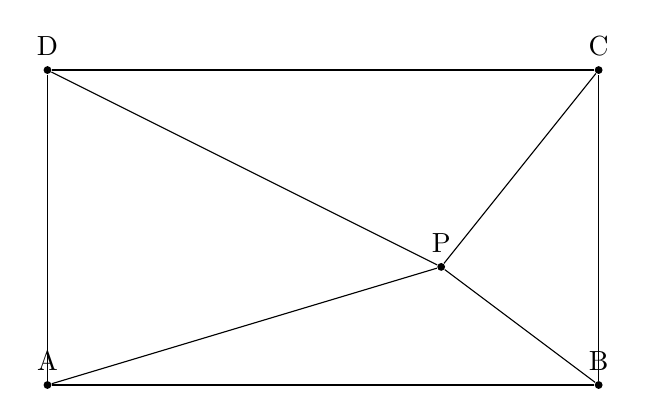
\begin{tikzpicture}[dot/.style={circle,inner sep=1pt,fill,label={#1},name=#1},
  extended line/.style={shorten >=-#1,shorten <=-#1},
  extended line/.default=1cm]
        \node [dot=A] at (0,0) {};
        \node [dot=B] at (7,0) {};
        \node [dot=C] at (7,4) {};
        \node [dot=D] at (0,4) {};
        \node [dot=P] at (5,1.5) {};
        \draw (A) -- (B) -- (C) -- (D) -- (A);
        \draw (P) -- (A);
        \draw (P) -- (B);
        \draw (P) -- (C);
        \draw (P) -- (D);
    \end{tikzpicture}
\end{figure}

\begin{proof}
This can be easily proven using Pythagoras' Theorem.
\end{proof}
\pagebreak

\section{Circle}
% https://yufeizhao.com/olympiad/cyclic_quad.pdf
The reader should be familiar with basic circle terminology, such as \vocab{centre}, \vocab{radius}, \vocab{chord}, \vocab{diameter}, \vocab{tangent}, \vocab{secant}, \vocab{arc}, \vocab{sector}, \vocab{segment}, and \vocab{circumference}.

\subsection{Angles}
\begin{itemize}
\item Angle subtended at the centre of a circle by a chord is twice the angle subtended on the circumference.
\item All angles subtended by a fixed chord in the same segment of a circle are equal.
\end{itemize}

\subsection{Cyclic Quadrilaterals}
Unlike triangles, not all quadrilaterals can be inscribed in a circle. Those which can be are known as \vocab{cyclic quadrilaterals}. Such quadrilaterals have the following special properties:
\begin{itemize}
\item Sum of opposite angles in a cyclic quadrilaterals is always $180\degree$.
\item When we draw the diagonals of a cyclic quadrilaterals, we form four pairs of equal inscribed angles.
\end{itemize}

% AOPS book 2 - Chapter 4 (pg 33)

Angle chasing and cyclic quadrilaterals
\begin{theorem}[Ptolemy's theorem]
Given a cyclic quadrilateral $ABCD$, the product of lengths of diagonals is equal to the sum of products of lengths of the pairs of the opposite sides: 
\begin{equation}
AC \cdot BD = AB \cdot CD + AD \cdot BC 
\end{equation} 
\end{theorem}

\begin{figure}[H]
\centering
\begin{asy}
import graph; size(6cm); real lsf=0.5; real xmin=-12.650403526770004,xmax=10.832004349475627,ymin=-7.279059049128651,ymax=2.9172496339779594; 
pair A=(-4.722835236346583,1.9593464813112522), B=(-0.13581566098455275,2.055853491787133), C=(1.9952034907831915,-3.715500660891391), D=(-6.4478295435721815,-4.230092924079331); 
draw(A--B--C--D--cycle); 
draw(A--C); draw(B--D);
draw(circle((-2.3441952074649755,-2.0386768685399885),4.652109101574643));
label("$A$",A,NW*lsf); label("$B$",B,NE*lsf); label("$C$",C,SE*lsf); label("$D$",D,SW*lsf); 
clip((xmin,ymin)--(xmin,ymax)--(xmax,ymax)--(xmax,ymin)--cycle);  
\end{asy}
\end{figure}

\begin{theorem}[Ptolemy's inequality]
For four points $A, B, C, D$ in the plane,
\begin{equation}
AB \cdot CD + BC \cdot DA \ge AC \cdot BD
\end{equation}
where equality holds if and only if $ABCD$ is a cyclic quadrilateral with diagonals $AC$ and $BD$ (or a trivial case where $A$, $B$, $C$ and $D$ are collinear.
\end{theorem}

\begin{proof}
We construct a point $P$ such that the triangles $APB$ and $DCB$ are similar and have the same orientation. This means that
\begin{equation} \tag{1}
BD = \frac{BA \cdot DC}{AP}
\end{equation}

But since this is a spiral similarity, we also know that the triangles $ABD$ and $PBC$ are also similar, which implies that
\begin{equation} \tag{2}
BD = \frac{BC \cdot AD}{PC}
\end{equation}

By the triangle inequality, we have $AP + PC \ge AC$. Multiplying both sides of the inequality by $BD$ and using equations $(1)$ and $(2)$ gives us
\[ BA \cdot DC + BC \cdot AD \ge AC \cdot BD \]

which is the desired inequality. Equality holds iff $A$, $P$, $C$ are collinear. But since the triangles $BAP$ and $BDC$ are similar, this would imply that the angles $BAC$ and $BDC$ are congruent, i.e. that $ABCD$ is a cyclic quadrilateral.
\end{proof}

\begin{theorem}[Brahmagupta's formula] 
Given a cyclic quadrilateral $ABCD$, 
\begin{equation}
[ABCD]=\sqrt{(s-a)(s-b)(s-c)(s-d)} 
\end{equation}
where $s$ denotes the semiperimeter.
\end{theorem}
\pagebreak

\subsection{Power of a Point} % https://cs.stanford.edu/~rayyli/static/contest/lectures/Ray%20Li%20pop.pdf
\textbf{Power of a point} is a frequently used tool in Olympiad geometry.

\begin{theorem}[Power of a point]
Let $\Gamma$ be a circle, and $P$ be a point. Let a line through $P$ meet $\Gamma$ at points $A$ and $B$, and another line through $P$ meet $\Gamma$ at points $C$ and $D$. Then 
\begin{equation}
PA \cdot PB = PC \cdot PD
\end{equation} 
\end{theorem}

\begin{figure}[H]
    \centering
    \includegraphics[width=12cm]{images/Power_of_a_point.png}
\end{figure}

\begin{proof}
There are two configurations to consider, depending on whether $P$ lies inside the circle or outside the circle.

When $P$ lies inside the circle, we have $\angle PAD = \angle PCB$ and $\angle APD = \angle CPB$, so triangles $PAD$ and $PCB$ are similar. Hence $\dfrac{PA}{PD} = \dfrac{PC}{PB}$. Rearranging, we get $PA \cdot PB = PC \cdot PD$.

When $P$ lies outside the circle, we have $\angle PAD = \angle PCB$ and $\angle APD = \angle CPB$, so again triangles $PAD$ and $PCB$ are similar. We get the same result in this case.
\end{proof}

As a special case, when $P$ lies outside the circle and $C=D$ ($PC$ is a tangent), we have \begin{equation} PA \cdot PB = PC^2 \end{equation}

\begin{figure}[H]
    \centering
    \includegraphics[width=6cm]{images/Power_of_a_point2.png}
\end{figure}
\pagebreak

\begin{theorem}[Converse to power of a point]
Let $A, B, C, D$ be four distinct points. Let lines $AB$ and $CD$ intersect at $P$. Assume that either (1) $P$ lies on both line segments $AB$ and $CD$, or (2) $P$ lies on neither line segments. Then $A, B, C, D$ are concyclic if and only if $PA \cdot PB = PC \cdot PD$.
\end{theorem}

\begin{proof}
The expression $PA \cdot PB = PC \cdot PD$ can be rearranged as $\dfrac{PA}{PD} = \dfrac{PC}{PB}$. In both configurations described in the statement of the theorem, we have $\angle APD = \angle CPB$. It follows by angles and ratios that triangles $APD$ and $CPB$ are similar.

Thus $\angle PAD = \angle PCB$. In both cases this implies that $A$, $B$, $C$ and $D$ are concyclic.
\end{proof}

\begin{definition}
Suppose that $\Gamma$ has centre $O$ and radius $r$. We say that the \vocab{power} of point $P$ with respect to $\Gamma$ is
\[ OP^2-r^2. \]
\end{definition}

Let line $PO$ meet $\Gamma$ at points $A$ and $B$, so that $AB$ is a diameter. We will use \emph{directed lengths}, meaning that for collinear points $P, A, B$, an expression such as $PA \cdot PB$ is assigned a positive value if $PA$ and $PB$ point in the same direction, and a negative value if they point in opposite directions. Then
\[ PA \cdot P B = (PO + OA)(PO + OB) = (PO-r)(PO+r) = PO^2-r^2, \]
which is the power of $P$. So the power of a point theorem says that this quantity equals to $PC \cdot PD$, where $C$ and $D$ are the intersections with $\Gamma$ of any line through $P$.

By convention, the power of $P$ is negative when $P$ is inside the circle, and positive when $P$
is outside the circle. When $P$ is outside the circle, the power equals to the square of the length
of the tangent from $P$ to the circle.

\begin{figure}[H]
    \centering
    \includegraphics[width=8cm]{images/Power_of_a_point3.jpg}
\end{figure}

Let $\Gamma_1$ and $\Gamma_2$ be two circles with different centres $O_1$ and $O_2$, and radii $r_1$ and r$_2$ respectively.

\begin{definition}
The \vocab{radical axis} of $\Gamma_1$ and $\Gamma_2$ is the set of points with equal powers with respect to both circles.
\[ {PO_1}^2-{r_1}^2 = {PO_2}^2-{r_2}^2 \]
which can be represented as 
\[ pow(P, \Gamma_1) = pow(P, \Gamma_2). \]
\end{definition}

\begin{lemma}
The radical axis is a line perpendicular to the line connecting the circles' centres.
\end{lemma}

\begin{proof}
We first prove two lemmas.
\begin{lemma}
Let $P$ be a point in the plane, and let $P'$ be the foot of the perpendicular from $P$ to $O_1O_2$. Then \[ pow(P, \Gamma_1)-pow(P, \Gamma_2) = pow(P', \Gamma_1)-pow(P', \Gamma_2). \]
\end{lemma}
The proof of the lemma is an easy application of the Pythagorean Theorem.

\begin{lemma}
There is a unique point $P$ on line $O_1O_2$ such that $pow(P, O_1) = pow(P, O_2)$.
\end{lemma}

Proof: First show that $P$ lies between $O_1$ and $O_2$ via proof by contradiction, by using a bit of inequality theory and the fact that $O_1O_2 > r_1 + r_2$. Then, use the fact that $O_1P + PO_2 = O_1O_2$ (a constant) to prove the lemma.

The first lemma shows that every point on the plane can be equivalently mapped to a line on $O_1O_2$. The second lemma shows that only one point in this mapping satisfies the given condition. Combining these two lemmas shows that the radical axis is a line perpendicular to $\ell$, hence proved.
\end{proof}

When $\Gamma_1$ and $\Gamma_2$ intersect, the intersection points $A$ and $B$ both have a power of $0$ with respect to either circle, so $A$ and $B$ must lie on the radical axis. This shows that the radical axis \emph{coincides with the common chord} when the circles intersect.

To show that some point lies on the radical axis or the common chord, we can show that the point has \emph{equal powers with respect to the two circles}.

\begin{figure}[H]
    \centering
    \includegraphics[width=10cm]{images/Radical_axis.jpg}
    \caption{Radical axis}
\end{figure}

\begin{figure}[H]
    \centering
    \includegraphics[width=10cm]{images/Radical_center.jpg}
    \caption{Radical centre}
\end{figure}

\begin{theorem}[Radical axis theorem]
Given three circles, no two concentric, the three pairwise radical axes (which are non-parallel) are concurrent, at a point known as the radical centre.
\end{theorem}

\begin{proof}
Denote the three circles by $\Gamma_1, \Gamma_2, \Gamma_3$, and denote the radical axes of $\Gamma_i$ and $\Gamma_j$ by $\ell_{ij}$.

Suppose that the radical axes are not all parallel. Let $\ell_{12}$ and $\ell_{13}$ meet at $X$. Since $X$ lies on $\ell_{12}$, it has equal powers with respect to $\Gamma_1$ and $\Gamma_2$. Since X lies on $\ell_{13}$, it has equal powers with respect to $\Gamma_1$ and $\Gamma_3$. Therefore, $X$ has equal powers with respect to all three circles, and hence it must lie on $\ell_{23}$ as well.
\end{proof}

\subsection{Theorems}
\begin{theorem}[Hamilton's theorem]
For $\triangle ABC$ with circumcentre $O$ and orthocentre $H$,
\[ \overrightarrow{OH} = \overrightarrow{OA} + \overrightarrow{OB} + \overrightarrow{OC} \]
\end{theorem}

\begin{theorem}[Euler line]
Circumcentre $O$, the centroid $G$ and the orthocentre $H$ are collinear. We also have
\[GH=2OG\]
and
\[OI^2=R^2-2Rr.\]
\end{theorem}

\begin{figure}[H]
\centering
\begin{asy}
import graph; size(8cm); real lsf=0.5; pen dps=linewidth(0.7)+fontsize(10); defaultpen(dps); pen ds=black; real xmin=-10.190749488267803,xmax=2.1327044306677894,ymin=-5.404837089903882,ymax=2.8163349988738835; 
pair A=(-5.649772389356279,1.9593464813112522), B=(-7.46244948857524,-2.6753392837372125), C=(-0.42710735249361875,-2.0393655406135887), G=(-4.513109743475047,-0.9184527810131827), H=(-5.466468833129196,-0.06841527263166719), O=(-4.03643019864797,-1.3434715352039406); 
draw(A--B--C--cycle);  draw(circle((-4.036430198647971,-1.3434715352039408),3.675796495256074)); draw((xmin,-0.8916236469616956*xmin-4.942448149628765)--(xmax,-0.8916236469616956*xmax-4.942448149628765),red); 
label("$A$",A,N*lsf); label("$B$",B,SW*lsf); label("$C$",C,E*lsf); dot(G,linewidth(4.pt)+ds); label("$G$",G,NE*lsf); dot(H,linewidth(4.pt)+ds); label("$H$",H,NE*lsf); dot(O,linewidth(4.pt)+ds); label("$O$",O,NE*lsf); 
clip((xmin,ymin)--(xmin,ymax)--(xmax,ymax)--(xmax,ymin)--cycle);  
\end{asy}
\end{figure}

\begin{theorem}[Nine-point circle]
The midpoints of each side of the triangle, the feet of each altitude, and the midpoints of the line segments from each vertex to the orthocentre, all lie on a single circle.
\end{theorem}

The centre of this circle lies on the Euler line, at the midpoint between the orthocentre and circumcentre.

The radius of this circle is half the circumradius of the triangle.

\begin{figure}[H]
\centering
\begin{asy}
import graph; size(8cm); real lsf=0.5; pen ds=black; real xmin=-9.29991987799322,xmax=4.227854476335946,ymin=-2.582016893191067,ymax=3.3073835513057874; 
pair A=(-4.3010727599189025,2.646623812442647), B=(-6.237341479539152,-1.782075918603663), C=(1.0133669173366817,-1.8026745220038782), D=(-4.313669818746617,-1.787540894912733), F=(-5.081333386332044,0.8619851456466379), G=(-2.6119872811012352,-1.7923752203037706), H=(-1.6438529212911104,0.4219746452193843), I=(-5.269207119729027,0.43227394691949195); 
draw(A--B--C--cycle); 
draw(A--D); draw(B--(-3.2595890330248367,1.7746839480662215)); draw(C--F); draw(circle((-3.458037931575361,-0.10366039891128645),1.8887984146430965),red); 
label("$A$",A,N*lsf); label("$B$",B,SW*lsf); label("$C$",C,SE*lsf); dot(D,ds); label("$D$",D,SW*lsf); dot((-3.2595890330248367,1.7746839480662215),ds); label("$E$",(-3.2595890330248367,1.7746839480662215),NE*lsf); dot(F,ds); label("$F$",F,NW*lsf); dot(G,ds); label("$G$",G,SE*lsf); dot(H,ds); label("$H$",H,NE*lsf); dot(I,ds); label("$I$",I,W*lsf); 
clip((xmin,ymin)--(xmin,ymax)--(xmax,ymax)--(xmax,ymin)--cycle); 
\end{asy}
\end{figure}

\begin{theorem}[Simson line]
Let $P$ be a point on the circumcircle of $\triangle ABC$. Points $D,E,F$ are the feet of the perpendicular bisectors from $P$ to sides (or the extensions of) $AB,AC,BC$ respectively. Then $D,E,F$ are collinear.
\end{theorem}

\begin{figure}[H]
\centering
\begin{asy}
import graph; size(8cm); real lsf=0.5; pen ds=black; real xmin=-11.67954538469208,xmax=9.668098139167585,ymin=-4.858791244160047,ymax=4.410580285936885;
pair A=(-3.0618387621655723,3.2139886884152817), B=(-5.142297705587335,-1.379499869832753), C=(1.7170372266844143,-1.338302663032322), P=(-1.8556455955550775,-3.79185012983495), D=(-5.489473189178031,-2.1460358385528), F=(-1.8702522152840195,-1.3598479449660663); 
draw(A--B--C--cycle); 
draw(circle((-1.71982057252597,-0.16171080952667127),3.6326794410915353)); draw(B--D,dashed); draw(P--D); draw(P--F); draw(P--(1.0693209211634036,-0.7212970444110164)); draw(D--(1.0693209211634036,-0.7212970444110164),red); 
label("$A$",A,N*lsf); label("$B$",B,W*lsf); label("$C$",C,E*lsf); dot(P,ds); label("$P$",P,S*lsf); dot(D,ds); label("$D$",D,W*lsf); dot((1.0693209211634036,-0.7212970444110164),ds); label("$E$",(1.0693209211634036,-0.7212970444110164),NE*lsf); dot(F,ds); label("$F$",F,N*lsf); 
clip((xmin,ymin)--(xmin,ymax)--(xmax,ymax)--(xmax,ymin)--cycle);  
\end{asy}
\end{figure}

\begin{proof}
Proof of existence: It suffices to show that $\angle NMP+\angle PML=180\degree$. 

$PCAB$ is a cyclic quadrilateral, so $\angle PBA+\angle ACP=\angle PBN+\angle ACP=180\degree$. $PMNB$ is a cyclic quadrilateral (since $\angle PMB=\angle PNB=90\degree$), so $\angle PBN+\angle NMP=180\degree$. Hence $\angle NMP=\angle ACP$. Now $PLCM$ is cyclic, so $\angle PML=\angle PCL=180\degree-\angle ACP$.

Therefore $\angle NMP+\angle PML=\angle ACP+(180\degree-\angle ACP)=180\degree$.
\end{proof}

We now prove some properties regarding the Simson line.

The Simson line of a vertex of the triangle is the altitude of the triangle dropped from that vertex, and the Simson line of the point diametrically opposite to the vertex is the side of the triangle opposite to that vertex.
If P and Q are points on the circumcircle, then the angle between the Simson lines of P and Q is half the angle of the arc PQ. In particular, if the points are diametrically opposite, their Simson lines are perpendicular and in this case the intersection of the lines lies on the nine-point circle.

\begin{lemma}
Let $ABC$ be a triangle with orthocentre $H$ and circumcircle $\odot(ABC)$. Suppose $P\in\odot(ABC)$. Let $\gamma$ be Simson's line of $P$ wrt $ABC$.

Prove that $\gamma$ bisects $PH$.
\end{lemma}

\begin{proof}
Let $PA,PB,PC$ be the projections of $P$ on the sides $BC,AC,AB$; let $Q$ be the intersection between $AH$ and the Simson's line of $P$. We want to show that $HQ=PP_A$. If we call $H_A$ the symmetric of $H$ with respect to the $BC$ side, we have that $HA$ lies on the circumcircle of $ABC$, so, in order to prove that $HQ=PP_A$, it is sufficient to show that $PP_AQH_A$ is an isosceles trapezoid. Let $\theta=\widehat{P_C P_A B}=\widehat{P_B P_A C}$. Since $PP_AP_CB$ and $PP_ACP_B$ are cyclic quadrilaterals, we have $\theta=\widehat{P_C P B}=\widehat{P_B P C}$, too.

Now:
\[\widehat{P_A Q H_A}=\frac{\pi}{2}-\theta,\]
and:
\[\widehat{P H_A Q}=\widehat{P H_A A}=\widehat{P B A}=\widehat{P B P_C}=\frac{\pi}{2}-\theta.\]
Since $PP_A$ and $QH_A$ are both ortogonal to $BC$, $PP_AQH_A$ is an isosceles trapezoid and we have $PP_A=QH$.
\end{proof}

Given two triangles with the same circumcircle, the angle between the Simson lines of a point P on the circumcircle for both triangles does not depend of P.

\begin{theorem}[Miquel's theorem]
Let $ABC$ be a triangle, and let $X, Y, Z$ be points on lines $BC, CA, AB$ respectively. Assume that the six points $A, B, C, X, Y, Z$ are all distinct. Then the circumcircles of triangles $AYZ, BZX, CXY$ pass through a common point.
\end{theorem}

\begin{figure}[H]
\centering
\begin{asy}
import graph; size(8cm); real lsf=0.5; pen ds=black; real xmin=-10.647193519393634,xmax=4.272620939998431,ymin=-3.1737370566747436,ymax=3.3046034322717803; 
pair A=(-4.681638029546153,2.7008962037190067), B=(-6.535512335565544,-1.7072049239270888), C=(-0.08814947129810388,-1.666007717126658), X=(-5.45557620465073,0.8606432095814611), Y=(-2.506653486956552,0.6331978941719494), Z=(-3.2603364974088445,-1.6862772827887074), D=(-3.2431897895257977,-0.11518658185591212); 
draw(A--B--C--cycle); 
draw(circle((-3.93804793471393,1.3053008916287092),1.5813325090761299)); draw(circle((-4.903125898654128,-0.8827091442329125),1.8287916147406886)); draw(circle((-1.6790880103434862,-0.9178959325207675),1.758054799284159)); 
label("$A$",A,N*lsf);label("$B$",B,SW*lsf); label("$C$",C,SE*lsf); label("$X$",X,W*lsf); label("$Y$",Y,NE*lsf); label("$Z$",Z,S*lsf); dot(D,ds); label("$D$",D,N*lsf); 
clip((xmin,ymin)--(xmin,ymax)--(xmax,ymax)--(xmax,ymin)--cycle); 
\end{asy}
\end{figure}

\begin{proof}
The proof involves angle chasing.
\end{proof}

Generalising, the circumcircles of the four triangles in a cyclic quadrilateral are concurrent.
\pagebreak

\section*{Exercises}
\begin{prbm}[\acrshort{smo} Open 2005 Q2]
Circles $C_1$ and $C_2$ have radii $3$ and $7$ respectively. The circles intersect at distinct points $A$ and $B$. A point $P$ outside $C_2$ lies on the line determined by $A$ and $B$ at a distance of $5$ from the center of $C_1$. Point $Q$ is chosen on $C_2$ so that $PQ$ is tangent to $C_2$ at $Q$. Find the length of the segment $PQ$.
\end{prbm}

\begin{solution}
The point $P$ lies on the radical axis of $C_1$ and $C_2$, namely $AB$, and hence has equal power with respet to both circles. Thus $PQ^2=5^2-3^2=16$.
\end{solution}
\pagebreak

\begin{prbm}[\acrshort{smo} Open 2005 Q10]
It is known that the three sides of a triangle are consecutive positive integers and the largest angle is twice the smallest angle. Find the perimeter of this triangle.
\end{prbm}

\begin{solution}
Let $\angle C=2\angle A$ and $CD$ the bisector of $\angle C$. Let $BC=x-1$, $CA=x$, $AB=x+1$. Then $\triangle ABC\sim\triangle CBD$, which implied
\[ \frac{BD}{BC}=\frac{BC}{AB}\implies BD=\frac{(x-1)^2}{x+1} \]
and
\[ \frac{CD}{AC}=\frac{CB}{AB}\implies AD=CD=\frac{x(x-1)}{x+1}. \]
Since $AB=AD+BD$, we have
\[ \frac{x(x-1)}{x+1}+\frac{(x-1)^2}{x+1}=x+1. \]
The only positive solution to this equation is $x=5$. Hence the perimeter is $15$.
\end{solution}
\pagebreak

\begin{prbm}[\acrshort{mat} 2022]
100 circles all share the same centre, the $n$-th circle named as $C_n$. For each whole number $n$ between 1 and 99 inclusive, a tangent to circle $C_n$ intersects circle $C_{n+1}$ at two points, separated by a distance of 2.

Given that $C_1$ has radius 1, what is the radius of $C_{100}$?
\end{prbm}

\begin{solution}
The relationship between circle $C_n$ of radius $r_n$ and circle $C_{n+1}$ of radius $r_{n+1}$ is shown below.

\begin{figure}[H]
\centering
\begin{asy}
size(6cm);
draw(circle((0,0),5));
draw(circle((0,0),3));
dot((0,0));
dot((3,4));
draw((0,0)--(3,4));
label("$r_{n+1}$",(0,0)--(3,4),NW);
dot((3,0));
draw((0,0)--(3,0));
label("$r_n$",(0,0)--(3,0),S);
draw((3,4)--(3,-4));
label("$1$",(3,4)--(3,0),E);
label("$1$",(3,-4)--(3,0),E);
\end{asy}
\end{figure}

The tangent is perpendicular to the radius, so there is a right-angled triangle with hypotenuse $r_{n+1}$ and other sides $r_n$ and $1$. By Pythagoras, we have 
\[ {r_{n+1}}^2 = {r_n}^2 + 1. \]
Since ${r_1}^2 = 1$, we have ${r_2}^2 = 2$ and ${r_3}^2 = 3$ and so on, up to ${r_{100}}^2 = 100$, so the radius of $C_{100}$ is 10.
\end{solution}
\pagebreak

\begin{prbm}[\acrshort{tstst} P5]
Let $ABC$ be a triangle with incentre $I$. Let $D$ be a point on side $BC$ and let $\omega_B$ and $\omega_C$ be the incircles of $\triangle ABD$ and $\triangle ACD$, respectively. Suppose that $\omega_B$ and $\omega_C$ are tangent to segment $BC$ at points $E$ and $F$, respectively. Let $P$ be the intersection of segment $AD$ with the line joining the centers of $\omega_B$ and $\omega_C$. Let $X$ be the intersection point of lines $BI$ and $CP$ and let $Y$ be the intersection point of lines $CI$ and $BP$. Prove that lines $EX$ and $FY$ meet on the incircle of $\triangle ABC$.
\end{prbm}

\begin{solution}
(homothety): Let $Z$ be the diametrically opposite point on the incircle. We claim this is the desired intersection.

\begin{figure}[H]
\centering
\begin{asy}
import geometry; import graph; import olympiad;

size(8cm); pair A = dir(110); pair B = dir(210); pair C = dir(330);

draw(A--B--C--cycle,red); draw(incircle(A, B, C),  lightblue);

pair D = 0.35*B+0.65*C; draw(A--D, red);

pair I_B = incentre(A, B, D); pair I_C = incentre(A, C, D); pair E = foot(I_B, B, C); pair F = foot(I_C, B, C);

draw(incircle(A, B, D), heavygreen); draw(incircle(A, C, D), heavygreen); pair I = incentre(A, B, C);

pair P = extension(I_B, I_C, A, D); draw(I_B--I_C, heavygreen);

pair X = extension(B, I, C, P); pair Y = extension(C, I, B, P); pair Z = extension(E, X, F, Y); draw(B--I--C, red); draw(X--C, dotted+heavygreen); draw(Y--B, dotted+heavygreen); draw(E--Z--F, dashed+heavygreen);

pair T = extension(B, C, I_B, I_C); draw(I_C--T, dotted+heavygreen); draw(C--T, dotted+red); pair W = foot(I, B, C);

dot("$A$", A, dir(A)); dot("$B$", B, dir(270)); dot("$C$", C, dir(270)); dot("$D$", D, dir(D)); dot("$I_B$", I_B, dir(170)); dot("$I_C$", I_C, dir(30)); dot("$E$", E, dir(E)); dot("$F$", F, dir(F)); dot("$I$", I, dir(90)); dot("$P$", P, dir(250)); dot("$X$", X, dir(160)); dot("$Y$", Y, dir(20)); dot("$Z$", Z, dir(140)); dot("$T$", T, dir(T)); dot("$W$", W, dir(W));
\end{asy}
\end{figure}

Note that:
$P$ is the insimilicenter of $\omega_B$ and $\omega_C$
$C$ is the exsimilicenter of $\omega$ and $\omega_C$.
Thus by Monge theorem, the insimilicenter of $\omega_B$ and $\omega$ lies on line $CP$.

This insimilicenter should also lie on the line joining the centers of $\omega$ and $\omega_B$, which is $\overline{BI}$, hence it coincides with the point $X$. So $X \in \overline{EZ}$ as desired.
\end{solution}

\begin{solution}
(harmonic): Let $T = \overline{I_B I_C} \cap \overline{BC}$, and $W$ the foot from $I$ to $\overline{BC}$. Define $Z = \overline{FY} \cap \overline{IW}$. Because $\angle I_B D I_C = 90^{\circ}$, we have\[ -1 = (I_B I_C; PT) \overset{B}{=} (I I_C; YC) 	\overset{F}{=} (I\infty; ZW) \]So $I$ is the midpoint of $\overline{ZW}$ as desired.
\end{solution}

\begin{solution}
(outline, barycentric, Andrew Gu): Let $AD = t$, $BD = x$, $CD = y$ (so with Stewart). We then have $D = (0:y:x)$ and so\[ \overline{AI_B} \cap \overline{BC} = \left( 0 : y + \frac{tx}{c+t} : \frac{cx}{c+t} \right) \]hence intersection with $BI$ gives $I_B = (ax : cy+at : cx)$. Similarly, $I_C = (ay : by : bx+at)$.

Then, we can compute\[ P = \left( 2axy : y(at+bx+cy) : x(at+bx+cy) \right) \]since $P \in \overline{I_B I_C}$, and clearly $P \in \overline{AD}$. Intersection now gives\begin{align*} 	X &= \left( 2ax : at+bx+cy : 2cx \right) \\ 	Y &= \left( 2ay : 2by : at+bx+cy \right). \end{align*}From here one can check that the antipode\[ Q = \left( 4a^2 : -a^2+2ab-b^2+c^2 : -a^2+2ac-c^2+b^2 \right) \]lies on each of lines $EX$ and $FY$ (using Stewart's Theorem).
\end{solution}
\pagebreak

\begin{prbm}[\acrshort{australia} 2024 P2]
Let $ABCD$ be a cyclic quadrilateral. Point $P$ is on line $CB$ such that $CP=CA$and $B$ lies between $C$ and $P$. Point $Q$ is on line $CD$ such that $CQ=CA$ and $D$ lies between $C$ and $Q$. Prove that the incentre of triangle $ABD$ lies on line $PQ$.
\end{prbm}

\begin{proof}
Let $PQ$ intersect the angle bisector of $\angle{BAC}$ at $I'$. $APBI'$ is cyclic since $\angle{BPI'}=\frac{\angle{A}}{2}=\angle{PAI'}$. Then, $\angle{I'BA}=\angle{I'PA}=\frac{\angle{QCA}}{2}=\frac{\angle{B}}{2}$ so $I'=I$ and we are done.
\end{proof}

\chapter{Analytic Geometry}
\section{Trigonometry}
% https://www.ams.org/books/prb/025/prb025-endmatter.pdf
% https://mathematicalolympiads.files.wordpress.com/2012/08/103-trigonometry-problems-titu-andreescu-zuming-feng.pdf
\vocab{Trigonometric functions} describe how the ratio of lengths vary according to the angle between the lengths.

For a triangle $\triangle ABC$ with $\angle C=90\degree$, we define \vocab{sine} as
\begin{equation}
\sin A=\frac{a}{c}
\end{equation}
and \vocab{cosine} as
\begin{equation}
\cos A=\frac{b}{c}.
\end{equation}
We define \vocab{tangent} as the ratio of sine and cosine; that is,
\begin{equation}
\tan A=\frac{\sin A}{\cos A}=\frac{a}{b}.
\end{equation}
We also define the reciprocals of the above trigonometric functions: \vocab{cosecant}, \vocab{secant} and \vocab{cotangent} are the reciprocals of sine, cosine and tangent respectively.
\begin{equation}
\cosec A=\frac{1}{\sin A}
\end{equation}
\begin{equation}
\sec A=\frac{1}{\cos A}
\end{equation}
\begin{equation}
\cot A=\frac{1}{\tan A}
\end{equation}

\subsection{Pythagorean identities}
The following equation is known as the \vocab{Pythagorean identity}.
\begin{equation}\label{pythagorean_identity}
\sin^2 A + \cos^2 A = 1
\end{equation}
\begin{proof}
\[ \sin^2A+\cos^2A=\brac{\frac{a}{c}}^2+\brac{\frac{b}{c}}^2=\frac{a^2+b^2}{c^2} \]
By Pythagoras' Theorem, for a right-angled triangle, $a^2+b^2=c^2$. Hence we have our desired result.
\end{proof}
The following two equations are corollaries of \cref{pythagorean_identity}; they can be easily derived and shall be left as an exercise for the reader.
\[ \tan^2 A + 1 = \sec^2 A \]
\[ 1 + \cot^2 A = \cosec^2 A \]

\begin{exercise}
Compute $\sin^25\degree+\sin^210\degree+\cdots+\sin^290\degree$.
\end{exercise}
\begin{solution}
\begin{align*}
&\sin^25\degree+\sin^210\degree+\cdots+\sin^290\degree \\
&= (\sin^25\degree+\sin^285\degree) + \cdots + (\sin^240\degree+\sin^250\degree)+\sin^245\degree+\sin^290\degree \\
&= (\sin^25\degree+\cos^25\degree) + \cdots + (\sin^240\degree+\cos^240\degree)+\frac{1}{2}+1 \\
&= 8(1)+\frac{1}{2}+1 \\
&= \boxed{9\frac{1}{2}}
\end{align*}
\end{solution}

\begin{exercise}
Evaluate
\[ \tan10\degree\tan20\degree\tan30\degree\cdots\tan80\degree. \]
\end{exercise}
\begin{solution}
Writing this in terms of sines and cosines, we have
\[ \frac{\sin10\degree\sin20\degree\sin30\degree\cdots\sin80\degree}{\cos10\degree\cos20\degree\cos30\degree\cdots\cos80\degree}. \]
Applying $\sin x=\cos(90\degree-x)$ to each term in the numerator, we get
\[ \frac{\cos80\degree\cos70\degree\cos60\degree\cdots\cos10\degree}{\cos10\degree\cos20\degree\cos30\degree\cdots\cos80\degree}=\boxed{1} \]
\end{solution}

\subsection{Addition formulae}
\[ \sin (A \pm B) = \sin A \cos B \pm \cos A \sin B \]
\[ \cos (A \pm B) = \cos A \cos B \mp \sin A \sin B \]
\[ \tan (A \pm B) = \frac{\tan A \pm \tan B}{1 \mp \tan A \tan B} \]

\subsubsection{Double-angle formulae}
\[ \sin 2A = 2 \sin A \cos A \]
\[ \begin{split}
\cos 2A &= \cos^2 A-\sin^2 A \\
&= 2 \cos^2 A-2 \\
&= 2-2 \sin^2 A
\end{split} \]
\[ \tan 2A = \frac{2 \tan A}{1-\tan^2 A} \]

\subsubsection{Triple-angle formulae}
\[ \sin 3A = 3 \sin A-4 \sin^3 A \]
\[ \cos 3A = 4 \cos^3 A- 3 \cos A \]
\[ \tan 3A = \frac{3\tan A-\tan^3A}{1-3\tan^2A} \]

\subsubsection{Half-angle formulae}
The following formulae are corollaries of the double angle formulae:
\[ \sin \frac{A}{2} = \pm \sqrt{\frac{1-\cos A}{2}} \]
\[ \cos \frac{A}{2} = \pm \sqrt{\frac{1+\cos A}{2}} \]

\subsubsection{Multiple-angle formulae}
To generalise, multiple-angle formulae are given by
\[ \sin nA = \sum_{k=0}^n \binom{n}{k} \cos^kA \sin^{n-k}A \sin\frac{n-k}{2}\pi \]
\[ \cos nA = \sum_{k=0}^n \binom{n}{k} \cos^kA \sin^{n-k}A \cos\frac{n-k}{2}\pi \]

\subsubsection{Sum to product}
The sum-to-product formulae can be derived from the addition formulae.
\[ \sin A + \sin B = 2 \sin \frac{A+B}{2} \cos \frac{A-B}{2} \]
\[ \sin A-\sin B = 2 \cos \frac{A+B}{2} \sin \frac{A-B}{2} \]
\[ \cos A + \cos B = 2 \cos \frac{A+B}{2} \cos \frac{A-B}{2} \]
\[ \cos A-\cos B = -2 \sin \frac{A+B}{2} \sin \frac{A-B}{2} \]

\subsubsection{Product to sum}
The product-to-sum formulae can be, in turn, simply observed from the sum-to-product formulae.
\[ \sin A \cos B = \frac{1}{2}\sqbrac{\sin(A+B)+\sin(A-B)} \]
\[ \cos A\sin B=\frac{1}{2}\sqbrac{\sin(A+B)-\sin(A-B)} \]
\[ \cos A\cos B = \frac{1}{2}\sqbrac{\cos(A+B)+\cos(A-B)} \]
\[ \sin A\sin B = -\frac{1}{2}\sqbrac{\cos(A+B)-\cos(A-B)} \]

\subsection{R-formula}
It is rather difficult to immediately the amplitude of some function of a combination of trigonometric functions, given by $f(x)=a\sin\theta+b\cos\theta$. To do so, we combine the two trigonometric functions using the \vocab{R-formula}.
\[ a \sin \theta \pm b \cos \theta = \sin (\theta \pm \alpha) \]
\[ a \cos \theta \mp b \cos \theta = \cos (\theta \pm \alpha) \]
where $R = \sqrt{a^2 + b^2}$,
$\alpha = \tan^{-1} \dfrac{b}{a}$ where $0 < \alpha < \frac{\pi}{4}$.

\subsection{Sine and Cosine Rules}
\begin{theorem}[Sine rule] 
Given $\triangle ABC$,
\begin{equation}
\frac{a}{\sin A}=\frac{b}{\sin B}=\frac{c}{\sin C}=2R
\end{equation} 
where $R$ denotes the circumradius of $\triangle ABC$.
\end{theorem}

\begin{theorem}[Cosine rule]
Given $\triangle ABC$,
\begin{equation}
c^2=a^2+b^2-2ab\cos C
\end{equation} 
\end{theorem}

\begin{exercise}[Pythagorean inequality]
Use the law of cosines to justify the statement that if $a$, $b$ and $c$ are the sides of triangle $\triangle ABC$ and $a\le b\le c$, then $\triangle ABC$ is acute if $a^2+b^2>c^2$ and obtuse if $a^2+b^2<c^2$.
\end{exercise}
\begin{proof}
From the law of cosines,
\[ \cos C=\frac{c^2-a^2-b^2}{-2ab}. \]
If $c^2<a^2+b^2$, then the numerator of RHS is negative, so $\cos C$ is positive and $\angle C$ is acute. Similarly, if $c^2>a^2+b^2$, $\cos C$ is negative and $\angle C$ is obtuse.
\end{proof}
\pagebreak

\section{Hyperbolic Functions}
\subsection{Basics}
The three main hyperbolic functions are:
\begin{equation}
\sinh x = \frac{e^x-e^{-x}}{2}
\end{equation}
\begin{equation}
\cosh x = \frac{e^x+e^{-x}}{2}
\end{equation}
\begin{equation}
\tanh x = \frac{e^x-e^{-x}}{e^x+e^{-x}} = \frac{e^{2x}-1}{e^{2x}+1}
\end{equation}

It is easy to see that
\[ \sinh x + \cosh x = e^x \]

\subsection{Reciprocals and Inverses}
Again these functions all have their inverse functions:
\begin{equation}
\sinh^{-1} x = \arsinh x = \ln(x+\sqrt{x^2+1})
\end{equation}
$\arsinh x$ has domain $x \ge 1$.

\begin{equation}
\cosh^{-1} x = \arcosh x = \ln(x+\sqrt{x^2-1})
\end{equation}
$\arcosh x$ has domain $x \ge 1$.

\begin{equation}
\tanh^{-1} x = \artanh x = \frac{1}{2}\ln(1+x)-\frac{1}{2}\ln(1-x)
\end{equation}
$\artanh x$ has domain $-1<x<1$.

As well as their reciprocal functions:
\begin{equation}
\cosech x = \frac{1}{\sinh x}
\end{equation}
\begin{equation}
\sech x = \frac{1}{\cosh x}
\end{equation}
\begin{equation}
\coth x = \frac{1}{\tanh x}
\end{equation}

\subsection{Identities}
Hyperbolic function identities have very similar forms to the trigonometric identities. 

However there is one key difference outlined in \vocab{Osborn's rule}: all the identities for the hyperbolic functions are exactly the same as the trigonometric identities, except whenever a product of two $\sinh$ functions is present we put a minus sign in front. For example if a trigonometric formula involved a $\sin^2x$, then the corresponding hyperbolic formula would contain a $-\sinh^2x$ instead.

\begin{table}[H]
\centering
\begin{tabular}{c|c}
\hline\hline
Trigonometric & Hyperbolic \\
\hline
$\cos^2\theta + \sin^2\theta = 1$ & $\cosh^2x-\sinh^2x = 1$ \\
$\sin(A \pm B) = \sin A \cos B \pm \cos A \sin B$ & $\sinh(A \pm B) = \sinh A \cosh B \pm \cosh A \sinh B$ \\
$\cos(A \pm B) = \cos A \cos B \mp \sin A \sin B$ & $\cosh(A \pm B) = \cosh A \cosh B \mp \sinh A \sinh B$ \\
$\cos 2\theta = \cos^2\theta-\sin^2\theta$ & $\cosh 2\theta = \cosh^2\theta + \sinh^2\theta$ \\
$\sin 2\theta = 2 \sin\theta \cos\theta$ & $\sinh 2\theta = 2 \sinh\theta \cosh\theta$ \\
$1 + \tan^2\theta = \sec^2\theta$ & $1-\tanh^2\theta = \sech^2\theta$ \\
$1 + \cot^2\theta = \cosec^2\theta$ & $1-\coth^2\theta =-\cosech^2\theta$ \\
\hline\hline
\end{tabular}
\end{table}
\pagebreak

\section{Cartesian Geometry}
\subsection{Basics}
The coordinate plane is determined by two \vocab{axes} -- a horizontal $x$-axis and a vertical $y$-axis; both axes intersect at a point called the \vocab{origin}. Each point in the coordinate plane can be specified by an ordered pair of numbers $(x,y)$.

The \vocab{gradient} of a line with points $(x_1, y_1)$ and $(x_2, y_2)$ is given by
\begin{equation}
m = \frac{y_2-y_1}{x_2-x_1}
\end{equation}

Given gradient $m$ and $y$-intercept $c$, a line can be represented in the point-slope form:
\begin{equation}
y=mx+c
\end{equation}

Given gradient $m$ and a point on the line $(x_1,y_1)$, a line also can be represented as
\begin{equation}
y-y_1=m(x-x_1)
\end{equation}

For two parallel lines, they have the same gradients.

For two perpendicular lines, the product of the gradients is $-1$.

Distance between two points $(x_1,y_1)$ and $(x_2,y_2)$ is given by
\begin{equation}
d=\sqrt{(x_1-x_2)^2+(y_1-y_2)^2}
\end{equation}
which follows easily from Pythagoras' Theorem.

The distance from a point $(m,n)$ to the line $Ax+By+C=0$ is given by
\[ d=\frac{Am+Bn+C}{\sqrt{A^2+B^2}} \]

The distance between two parallel lines $Ax+By+C_1=0$ and $Ax+By+C_2=0$ is given by
\[ d=\frac{|C_2-C_1|}{\sqrt{A^2+B^2}} \]

Using the \vocab{shoelace formula}, the area of a polygon is given by


The reflection of point/line about line

\subsection{Conic Sections}
%Definitions and basic properties of conic sections - refer to F maths
%AOPS book 2 Chap 5
\vocab{Conic sections} are the family of curves obtained by intersecting a cone with a plane. This intersection can take different forms according to the angle the intersecting plane makes with the side of the cone. 

The standard conic sections are\footnote{There are also special cases, such as a point or a line, however these are trivial (sometimes called degenerate) so we shall not cover them.}
\begin{enumerate}
\item \textbf{circle}
\item \textbf{parabola}
\item \textbf{ellipse}
\item \textbf{hyperbola}
\end{enumerate}

\begin{table}[H]
\centering
\renewcommand{\arraystretch}{1.8}
\begin{tabular}{c|c|c}
\hline\hline
Conic & Cartesian equation & Parametric equation \\
\hline
Circle & $x^2+y^2=a^2$ & $x=\cos t, y=\sin t$ \\
Parabola & $x=4ay^2$ & $x=4at^2, y=t$ \\
Ellipse & $\frac{x^2}{a^2}+\frac{y^2}{b^2}=1$ & $x=a\cos t, y=b\sin t$ \\
Hyperbola & $\frac{x^2}{a^2}-\frac{y^2}{b^2}=1$ & $x=b\tan t, y=a\sec t$ \\
\hline\hline
\end{tabular}
\end{table}

\begin{remark}
The circle is a special case of the ellipse, where $a=b$.
\end{remark}

\subsubsection{Parabolas}
Given a line $l$ and a point $P$ in a plane, a \textbf{parabola} is defined as the set of points $S$ in the plane such that the length $SP$ equals the distance from $S$ to $l$. The point $P$ is known as the \vocab{focus}, and the line $l$ is known as the \vocab{directrix}.

[figure]

The minimum point on the curve is known as the \vocab{vertex}, denoted by $X(h,k)$.

If we let the distance from $X$ to $P$ be $a$, we have $P(h,k+a)$. Similarly, $l$ is $a$ below $X$ (since $X$ is equidistant from $P$ and $l$) and thus can be described by $y=k-a$. (Remember, $l$ is a horizontal line.) If we choose any point $S=(x,y)$ on the parabola, we have $SP=\sqrt{(x-h)^2+(y-k-a)^2}$ and the distance from $S$ to $l$ is simply $y-(k-a)$, or $y-k+a$. Hence from our definition of a parabola we have 
\[ \sqrt{(x-h)^2+(y-k-a)^2}=y-k-a. \]
Through some algebraic manipulation we have 
\begin{equation}
y-k=\frac{1}{4a}(x-h)^2
\end{equation}
which is the general form of a parabola with a horizontal directrix.

Similarly, if the directrix is vertical, the equation is
\[ x-h=\frac{1}{4a}(y-k)^2 \]

The \vocab{axis of symmetry} is the line through the focus and the vertex.

\subsubsection{Ellipses}
The general equation for a circle with radius $R$ is
\begin{equation}
(x-h)^2+(y-k)^2=R^2
\end{equation}
Dividing both sides by $R^2$, we can write this as 
\[ \frac{(x-h)^2}{R^2}+\frac{(y-k)^2}{R^2}=1. \]
Notice that we can ``stretch'' a circle to form an ellipse. Let $a$ denote the ``radius'' in the $x$-direction and $b$ denote the ``radius'' in the $y$-direction. Then the equation of an ellipse is given by
\begin{equation}\label{eqn:ellipse}
\frac{(x-h)^2}{a^2}+\frac{(y-k)^2}{b^2}=1
\end{equation}
Notice we have two different ``diameters'' in the $x$ and $y$ directions. These are known as the \vocab{major axis} and \vocab{minor axis}, where the major axis is the longer of the two.

Taking two points $F_1$ and $F_2$, known as \vocab{foci}, we can define an \vocab{ellipse} as the set of points $Z$ such that $ZF_1+ZF_2$ is constant.

We measure the amount an ellipse is stretched away from a circle by its \vocab{eccentricity} $e$. Let $c$ denote distance from centre of ellipse to either focus.
\begin{equation}
e=\frac{c}{a}
\end{equation}

The area enclosed in an ellipse is $ab\pi$.

\subsubsection{Hyperbolas}
The general form of the equation for a hyperbola is 
\begin{equation}
\frac{(x-h)^2}{a^2}-\frac{(y-k)^2}{b^2}=1
\end{equation}
With each hyperbola we can associate a pair of \vocab{foci} $F_1$ and $F_2$ so that the hyperbola is the set of all points $S$ where $|SF_1-SF_2|$ is constant.
\pagebreak

\subsection{Polar Coordinates}
You will already be familiar with coordinates in the form $(x, y)$ meaning that we move $x$ units in the $x$-direction (along the $x$-axis) and $y$ in the $y$-direction (along the $y$-axis). These are Cartesian coordinates on the $xy$-plane. Although Cartesian coordinates are very useful, there are sometimes situations where it is much easier to use another coordinate system called \vocab{polar coordinates}. These are coordinates in the form $(r,\theta)$ where $r$ is the distance to the point from the origin and $\theta$ is the angle in radians between the positive $x$-axis and the line formed by $r$.

From trigonometry and Pythagoras' theorem there are the following relationships:
\[ x = r\cos\theta \quad y = r\sin\theta \quad r = \sqrt{x^2+y^2} \]
We can use the formulae above to allow us to convert between polar and Cartesian coordinates.

Polar Coordinates, Parametric Equations and Vector Functions: polar coordinate system. Parametric equations are introduced. Derivatives and integrals of polar, parametric and vector functions will also be taught.
\pagebreak

\section{Linear Algebra}
%https://artofproblemsolving.com/wiki/index.php/Linear_algebra

A matrix over a field $F$ is a function from $A\times B$ to $F$, where $A$ and $B$ are the sets $A=\{1,2,\ldots,m\}$ and $B=\{1,2,\ldots,n\}$. A matrix is usually represented as a rectangular array of scalars from the field, such that each column belongs to the vector space $F^m$, where $m$ is the number of rows. If a matrix $A$ has $m$ rows and $n$ columns, its order is said to be $m \times n$, and it is written as $A_{m \times n}$.

The element in the $i^{th}$ row and $j^{th}$ column of $A$ is written as $(A)_{ij}$. It is more often written as $a_{ij}$, in which case $A$ can be written as $[a_{ij}]$.

\subsection{Determinant}
If $A_{m\times n}$ is a matrix over $F$ with $m=n$, a Determinant assigns $A_{m\times n}$ to a member of $F$ and is denoted by $|A|$ or $\begin{vmatrix} a_{11} & a_{12} & \ldots & a_{1n} \\ a_{21} & a_{22} & \ldots & a_{2n} \\ \vdots & \vdots & \ddots & \vdots \\ a_{n1} & a_{n2} & \ldots & a_{nn}\end{vmatrix}$

It is defined recursively.

$\begin{vmatrix} a_{11} & a_{12} \\ a_{21} & a_{22} \end{vmatrix}\dot{=}a_{11} a_{22}-a_{21} a_{12}$ $\begin{vmatrix} a_{11} & a_{12} & \ldots & a_{1n} \\ a_{21} & a_{22} & \ldots & a_{2n} \\ \vdots & \vdots & \ddots & \vdots \\ a_{n1} & a_{n2} & \ldots & a_{nn}\end{vmatrix}\dot{=}\sum_{k=1}^n (-1)^{k+1} a_{1k} |A'_{1k}|$
where $A'_{cd}$ is the matrix $A$ with the $c^{th}$ row and $d^{th}$ column removed.

\subsection{Transposes}
Let $A$ be $[a_{ij}]$. Then $[a_{ji}]$ is said to be the transpose of $A$, written as $A^T$ or simply $A'$. If A is over the complex field, replacing each element of $A^T$ by its complex conjugate gives us the conjugate transpose $A^*$ of $A$. In other words, $A^*=[\bar {a_{ji}}]$

$A$ is said to be symmetric if and only if $A=A^T$. $A$ is said to be hermitian if and only if $A=A^*$. $A$ is said to be skew symmetric if and only if $A=-A^T$. $A$ is said to be skew hermitian if and only if $A=-A^*$.

\subsection{Matrix Product}
Let $A$ be a matrix of order $m_1 \times m_2$ and $B$ a matrix of order $n_1 \times n_2$. Then the product $AB$ exists if and only if $m_2=n_1$ and in that case we define the product $C=AB$ as the matrix of order $m_1 \times n_2$ for which\[(C)_{ij}=\sum ^{n_1} _{k=1} (A)_{ik} (B)_{kj}\]for all $i$ and $j$ such that $1\le i\le m_1$ and $1\le j\le n_2$.

\subsection{Vector spaces associated with a matrix}
As already stated before, the columns of $A$ form a subset of $F^m$. The subspace of $F^m$ generated by these columns is said to be the column space of $A$, written as $C(A)$. Similarly, the transposes of the rows form a subset of the vector space $F^n$. The subspace of $F^n$ generated by these is known as the row space of $A$, written as $R(A)$.

$y \in C(A)$implies $\exists x$ such that $y_{m \times 1} = A_{m \times n} x_{n \times 1}$

Similarly, $y \in C(A)$implies $\exists x$ such that $y_{n \times 1} = A^T_{n \times m} x_{m \times 1}$

The set $\{x:A_{m \times n}x_{n \times 1} = \phi\}$ forms a subspace of $F^n$, known as the null space $N(A)$ of $A$.

\subsection{Rank and nullity}
The dimension of $C(A)$ is known as the column rank of $A$. The dimension of $R(A)$ is known as the row rank of $A$. These two ranks are found to be equal, and the common value is known as the rank $r(A)$ of $A$.

The dimension of $N(A)$ is known as the nullity $\eta (A)$ of A.

If $A$ is a square matrix of order $n \times n$, then $r(A) + \eta (A) = n$.
\pagebreak

\section{Complex Numbers}
%https://artofproblemsolving.com/wiki/index.php/Complex_numbers
\pagebreak

\section{Barycentric Coordinates}
%https://artofproblemsolving.com/wiki/index.php/Barycentric_coordinates
\subsection{The Basics}
$\triangle ABC$ is a fixed non-degenerate reference triangle with vertices in counterclockwise order. The lengths will be abbreviated $a=BC$, $b=CA$, $c=AB$. These correspond with points in the vector plane $\vec{A}, \vec{B}, \vec{C}$.

For arbitrary points $P$, $Q$ and $R$, $[PQR]$ denotes the signed area of $\triangle PQR$.

\subsubsection{The Coordinates}
\begin{definition}
Each point in the plane is assigned an ordered triple of real numbers $P=(x,y,z)$ such that
\[ \vec{P} = x\vec{A} + y\vec{B} + z\vec{C} \quad \text{and} \quad x + y + z = 1. \]
These are called the \vocab{barycentric coordinates} of the point.
\end{definition}

These are sometimes called areal coordinates because if $P=(x,y,z)$, then the signed area $[CPB]$ is equal to $x[ABC]$, and so on. In other words, these coordinates can be viewed as
\[P=\frac{1}{[ABC]}\brac{[PBC],[PCA],[PAB]}.\]
Of course, notice that $A=(1,0,0)$, $B=(0,1,0)$ and $C=(0,0,1)$! This is why barycentric coordinates are substantially more suited for standard triangle geometry problems.

\subsubsection{Lines}
\begin{theorem}[Line]
The equation of a line is
\[ux+vy+wz=0\]
where $u,v,w$ are reals.
\end{theorem}

In particular, if a line $\ell$ passes through a vertex, say $A$, then
\[u(1)+v(0)+w(0)=0\implies u=0.\]
So we rearrange to obtain

\begin{corollary}[Line through a vertex]
The equation of a line passing through $A$ is simply of the
form $y=kz$ for some constant $k$.
\end{corollary}

In particular, the equation for the line $AB$ is simply $z=0$, by substituting $(1,0,0)$ and $(0,1,0)$ into $ux+vy+wz=0$.

In fact, the above techniques are already sufficient to prove both Ceva's and Menelaus's Theorem:

\begin{theorem}[Ceva's theorem]
Let $AD$, $BE$ and $CF$ be cevians of $\triangle ABC$. Then the cevians concur if and only if
\[\frac{BD}{DC}\frac{CE}{EA}\frac{AF}{FB}=1.\]
\end{theorem}

\begin{proof}
Since $D$ lies on $BC$, the point $D$ has the form $D=(0,d,1-d)$. So the equation of line $AD$ is simply
\[z=\frac{1-d}{d}y.\]
Similarly, if we let $E=(1-e,0,e)$ and $F=(f,1-f,0)$ then the lines $BE$ and $CF$ have equations $x=\dfrac{1-e}{e}z$ and $y=\dfrac{1-f}{f}x$ respectively.

Notice that this system of three equations is homogeneous, so we may ignore the condition that $x+y+z=1$ temporarily. Then it is easy to see that this equation has solutions if and only if
\[\frac{(1-d)(1-e)(1-f)}{def}=1.\]
\end{proof}

Menelaus’s Theorem

\subsubsection{Special points}
Here we give explicit forms for several special points in barycentric coordinates. It will be understood that $(u:v:w)$ refers to the point $\dfrac{1}{u+v+w}(u,v,w)$; that is, we are not normalizing the coordinates such that they sum to $1$.

Again, the coordinates here are not homogenised!

\begin{table}[H]
\centering
\begin{tabular}{p{0.3\linewidth}p{0.6\linewidth}}
\hline\hline
\textbf{Point} & \textbf{Coordinates} \\
\hline
Centroid & $G=(1:1:1)$ \\
Incentre & $I=(a:b:c)$ \\
Symmedian point & $K:(a^2:b^2:c^2)$ \\
Excentre & $I_a=(-a:b:c)$, etc. \\
Orthocentre & $H=(\tan A:\tan B:\tan C)$ \\
Circumcentre & $O=(\sin2A:\sin2B:\sin2C)$ \\
\hline\hline
\end{tabular}
\end{table}

\subsection{Standard Strategies}
\subsubsection{Perpendicular lines}
%https://s3.amazonaws.com/aops-cdn.artofproblemsolving.com/resources/articles/bary.pdf
% https://web.evanchen.cc/handouts/bary/bary-full.pdf
\pagebreak

\section*{Exercises}
\begin{prbm}[\acrshort{smo} Open 2023 Q11]
Let $ABC$ be a triangle satisfying the following conditions that $\angle A+\angle C=2\angle B$ and $\dfrac{1}{\cos A}+\dfrac{1}{\cos C}=\dfrac{-\sqrt{2}}{\cos B}$. Determine the value of $\cos\dfrac{A-C}{2}$.
\end{prbm}

\begin{solution}
Given that $\angle A+\angle C=2\angle B$, we can easily see that $\angle B=60\degree \implies \cos B=\dfrac{1}{2}$ and $\angle A+\angle C=120\degree$.
\begin{align*}
\frac{1}{\cos A}+\frac{1}{\cos C} &= -2\sqrt{2} \\
\cos A+\cos C &= -2\sqrt{2}\cos A\cos C
\end{align*}
Applying sum-to-product to the LHS and product-to-sum to the RHS gives
\[ 2\cos\frac{A+C}{2}\cos\frac{A-C}{2}=-\sqrt{2}\sqbrac{\cos(A+C)+\cos(A-C)} \]
Let $x=\cos\dfrac{A-C}{2}$. Then since $A+C=120\degree$,
\begin{align*}
&x=-\sqrt{2}\brac{-\frac{1}{2}+2x^2-1} \\
&2\sqrt{2}x^2+x-\frac{3}{2}\sqrt{2}=0 \\
&x=-\frac{3}{\sqrt{2}}\text{ (rej.)} \quad \text{or} \quad x=\frac{1}{\sqrt{2}}
\end{align*}
\end{solution}

\begin{prbm}[\acrshort{smo} Open 2023 Q19]
Let $ABC$ be a triangle with $AB=c$, $AC=b$ and $BC=a$, and satisfies the conditions $\tan C=\dfrac{\sin A+\sin B}{\cos A+\cos B}$, $\sin(B-A)=\cos C$ and area of triangle $ABC$ is $3+\sqrt{3}$. Determine the value of $a^2+c^2$.
\end{prbm}

\begin{solution}
\[ \tan C=\frac{\sin A+\sin B}{\cos A+\cos B}=\frac{2\sin\frac{A+B}{2}\cos\frac{A-B}{2}}{2\cos\frac{A+B}{2}\cos\frac{A-B}{2}}=\frac{\sin\frac{A+B}{2}}{\cos\frac{A+B}{2}}=\tan\frac{A+B}{2} \iff C=\frac{A+B}{2} \]
Since $A+B=180\degree-C$, we then have $C=60\degree$.

\[ \sin(B-A)=\cos C=\cos(180\degree-A-B)=\sin(A+B-90\degree) \]
which implies that $B-A=A+B-90\degree$. Thus $A=45\degree, B=75\degree$.

Given the area of the triangle,
\begin{align*}
3+\sqrt{3}&=\frac{1}{2}ac\sin B\\
&=\frac{1}{2}ac\sin(45\degree+30\degree) \\
&= \frac{1}{2}ac(\sin45\degree\cos30\degree+\cos45\degree\sin30\degree)\\
&=\frac{1}{2}ac\brac{\frac{1+\sqrt{3}}{2\sqrt{2}}}
\end{align*}
Hence
\[ ac=\frac{4\sqrt{2}(3+\sqrt{3})}{1+\sqrt{3}}=4\sqrt{6}. \]
By Sine Rule, we have $\dfrac{a}{\sin A}=\dfrac{c}{\sin C}$, giving us $\dfrac{a}{\sqrt{2}}=\dfrac{c}{\sqrt{3}}$. Hence 
\[ a\brac{\frac{\sqrt{3}a}{\sqrt{2}}}=4\sqrt{6}\implies a^2=8 \quad \text{and} \quad \brac{\frac{\sqrt{2}c}{\sqrt{3}}}=4\sqrt{6}\implies c^2=12. \]
This gives us $a^2+c^2=20$.
\end{solution}

\begin{prbm}[\acrshort{smo} Open 2021 Q1]
Given that $\dfrac{\pi}{2}<\beta<\alpha<\dfrac{3\pi}{4}$, $\cos(\alpha-\beta)=\dfrac{12}{13}$ and $\sin(\alpha+\beta)=-\dfrac{3}{5}$. Find $\sin2\alpha$.
\end{prbm}

\begin{solution}
Note that $\alpha-\beta$ is in the first quadrant and $\alpha+\beta$ is in the third quadrant.
\begin{align*}
\sin2\alpha&=\sin[(\alpha+\beta)+(\alpha-\beta)] \\
&=\sin(\alpha+\beta)\cos(\alpha-\beta)+\cos(\alpha+\beta)\sin(\alpha-\beta) \\
&= \brac{-\frac{3}{5}}\brac{\frac{12}{13}}+\brac{-\frac{4}{5}}\brac{\frac{5}{13}}=\boxed{-\frac{56}{65}}
\end{align*}
\end{solution}

\begin{prbm}[\acrshort{smo} Open 2018 Q13]
Let $\triangle ABC$ be a triangle with $a=BC$, $b=AC$ and $c=AB$. Given that $a+c=2b$, $\angle A-\angle C=\dfrac{\pi}{3}$, find $\sin B$.
\end{prbm}

\begin{solution}
From Sine rule,
\[ \frac{a}{\sin A}=\frac{b}{\sin B}=\frac{c}{\sin C}. \]
Since $a+c=2b$, we have
\[ 2\sin B=\sin A+\sin C \]
or
\[ 2\brac{2\sin\frac{B}{2}\cos\frac{B}{2}}=2\sin\frac{A+C}{2}\cos\frac{A-C}{2}. \]
Since $A+B+C=\pi$,
\[ 2\sin\frac{A+C}{2}\cos\frac{A-C}{2}=2\sin\frac{\pi-B}{2}\cos\frac{\frac{\pi}{3}}{2}=2\cos\frac{B}{2}\frac{\sqrt{3}}{2}. \]
Hence we have $\sin\dfrac{B}{2}=\dfrac{\sqrt{3}}{4}$ and thus $\cos\dfrac{B}{2}=\dfrac{\sqrt{13}}{4}$. Therefore
\[ \sin B=2\sin\frac{B}{2}\cos\frac{B}{2}=\boxed{\frac{\sqrt{39}}{8}}. \]
\end{solution}

\begin{prbm}[\acrshort{smo} Open 2013 Q9]
Let $A = \cos^2 10\degree+\cos^2 50\degree-\sin40\degree\sin80\degree$. Determine the value of $A$.
\end{prbm}
\begin{solution}
Let $B=\sin^210\degree+\sin^250\degree-\cos40\degree\cos80\degree$.

Then
\begin{align*}
A+B &= 2-\cos40\degree \\
A-B &= (\cos^210\degree-\sin10\degree) + (\cos^250\degree-\sin^250\degree) + (\cos40\degree\cos80\degree-\sin40\degree\sin80\degree) \\
&= \cos20\degree + \cos100\degree + \cos(40\degree+80\degree) \\
&= \cos20\degree + \cos100\degree + \cos120\degree \\
&= 2\cos60\degree\cos40\degree-\cos60\degree \\
&= \cos40\degree-\frac{1}{2}
\end{align*}
Adding up the two equations gives us $2A=\dfrac{3}{2}$. Hence $\boxed{A=\dfrac{3}{4}}$.
\end{solution}

\begin{prbm}[\acrshort{smo} Open 2011 Q16]
Determine the value of $\dfrac{3}{\sin^220\degree}-\dfrac{1}{\cos^220\degree}+64\sin^220\degree$.
\end{prbm}

\begin{solution}
\begin{align*}
&\frac{3}{\sin^220\degree}-\frac{1}{\cos^220\degree}+64\sin^220\degree \\
&= \frac{6}{1-\cos40\degree}-\frac{2}{1+\cos40\degree}+32(1-\cos40\degree) \quad \text{[double angle formula]} \\
&= \frac{6(1+\cos40\degree)}{1-\cos^240\degree}-\frac{2(1-\cos40\degree)}{1-\cos^240\degree}-32\cos40\degree+32 \\
&= \frac{4(1-6\cos40\degree+8\cos^340\degree)}{1-\cos^240\degree}+32 \\
&= \frac{4(1+2(4\cos^340\degree-3\cos40\degree))}{1-\cos^240\degree}+32 \\
&= \frac{4\brac{1+2\cos3(40\degree)}}{1-\cos^240\degree}+32 \quad \text{[triple angle formula]} \\
&=\frac{4\brac{1-2\brac{\frac{1}{2}}}}{1-\cos^240\degree}=\boxed{32}
\end{align*}
\end{solution}

\begin{prbm}[\acrshort{smo} Open 2009 Q1]
Evaluate the expression $\sin10\degree\cos20\degree\cos30\degree\cos40\degree$.
\end{prbm}

\begin{solution}

\end{solution}

\begin{prbm}[\acrshort{smo} Open 2009 Q6]
Find the value of $\dfrac{\sin80\degree}{\sin20\degree}-\dfrac{\sqrt{3}}{2\sin80\degree}$.
\end{prbm}

\begin{solution}

\end{solution}

\begin{prbm}[\acrshort{smo} Open 2009 Q22]
Evaluate $\displaystyle\sum_{k=0}^\infty\frac{2}{\pi}\tan^{-1}\frac{2}{(2k+1)^2}$.
\end{prbm}

\begin{solution}
We can rewrite the fraction as
\[ \frac{2}{(2k+1)^2}=\frac{2}{4k^2+4k+1}=\frac{2k+2-2k}{1+2k(2k+2)} \]
which is in the same form as $\tan(A-B)=\dfrac{\tan A-\tan B}{1+\tan A\tan B}$. Thus
\[ \tan\brac{\tan^{-1}(2k+2)-\tan^{-1}(2k)}=\frac{2k+2-2k}{1+2k(2k+2)}. \]
Therefore
\begin{align*}
\sum_{k=0}^\infty\frac{2}{\pi}\tan^{-1}\frac{2}{(2k+1)^2}
&= \frac{2}{\pi}\sum_{k=0}^\infty\tan^{-1}\tan\brac{\tan^{-1}(2k+2)-\tan^{-1}(2k)} \\
&= \frac{2}{\pi}\sum_{k=0}^\infty\brac{\tan^{-1}(2k+2)-\tan^{-1}(2k)} \\
&= \frac{2}{\pi}\lim_{n\to\infty}\sum_{k=0}^n\brac{\tan^{-1}(2k+2)-\tan^{-1}(2k)} \\
&= \frac{2}{\pi}\lim_{n\to\infty}\brac{-\tan^{-1}0+\tan^{-1}(2n+2)} \quad \text{[telescoping sum]} \\
&= \frac{2}{\pi}\lim_{n\to\infty}\tan^{-1}(2n+2) \\
&= \frac{2}{\pi}\brac{\frac{\pi}{2}}=\boxed{1}
\end{align*}
\end{solution}

\begin{prbm}[\acrshort{smo} Open 2006 Q16]
Find the value of 
\[ \frac{400(\cos^515\degree+\sin^515\degree)}{\cos15\degree+\sin15\degree}. \]
\end{prbm}

\begin{solution}
\begin{align*}
&\frac{400(\cos^515\degree+\sin^515\degree)}{\cos15\degree+\sin15\degree} \\
&= 400(\cos^415\degree-\cos^315\degree\sin15\degree+\cos^215\degree\sin^215\degree-\cos15\degree\sin^315\degree+\sin^415\degree) \\
&= 400(\cos^415\degree+\sin^415\degree-\cos15\degree\sin15\degree+\cos^215\degree\sin^215\degree) \\
&= 400\brac{(\cos^215\degree+\sin^215\degree)^2-\cos^215\degree\sin^215\degree-\cos15\degree\sin15\degree} \\
&= 400\sqbrac{1-\brac{\frac{1}{2}\sin30\degree}^2-\brac{\frac{1}{2}\sin30\degree}}=\boxed{275}
\end{align*}
\end{solution}

\begin{prbm}[\acrshort{smo} Open 2018]
Find the value of
\[ \frac{\tan40\degree\tan60\degree\tan80\degree}{\tan40\degree+\tan60\degree+\tan80\degree}. \]
\end{prbm}
\begin{solution}
We can show, more generally, that an acute $\triangle ABC$,
\[ \frac{\tan A\tan B\tan C}{\tan A+\tan B+\tan C}=1. \]
We see that
\begin{align*}
\tan A+\tan B+\tan 
&= \tan A+\tan B+\tan[180\degree-(A+B)] \\
&= \tan A+\tan B-\tan(A+B) \\
&= \tan A+\tan B-\frac{\tan A+\tan B}{1-\tan A\tan B} \\
&= (\tan A+\tan B)\brac{1-\frac{1}{1-\tan A\tan B}} \\
&= (\tan A+\tan B)\brac{-\frac{\tan A\tan B}{1-\tan A\tan B}} \\
&= \tan A\tan B\brac{-\frac{\tan A+\tan B}{1-\tan A\tan B}} \\
&= \tan A\tan B[-\tan(A+B)] \\
&= \tan A\tan B\tan[180\degree-(A+B)] \\
&= \tan A\tan B\tan C
\end{align*}
Hence proven.
\end{solution}
\pagebreak

\begin{prbm}
Angles of $\triangle ABC$ satisfies
\[ \frac{\sin A+\sin B+\sin C}{\cos A+\cos B+\cos C}=\frac{12}{7} \]
and
\[ \sin A\sin B\sin C=\frac{12}{15}. \]
Given that $\sin C$ takes on three possible values $s_1,s_2,s_3$, find the value of $s_1s_2s_3$.
\end{prbm}
\begin{solution} \
\begin{align*}
\sin A+\sin B+\sin C
&= 2\sin\frac{A+B}{2}\cos\frac{A-B}{2}+\sin C \\
&= 2\sin\brac{90\degree-\frac{C}{2}}\cos\frac{A-B}{2}+2\sin\frac{C}{2}\cos\frac{C}{2} \\
&= 2\cos\frac{C}{2}\cos\frac{A-B}{2}+2\sin\frac{C}{2}\cos\frac{C}{2} \\
&= 2\cos\frac{C}{2}\brac{\cos\frac{A-B}{2}+\cos\frac{A+B}{2}} \\
&= 2\cos\frac{C}{2}\brac{2\cos\frac{A}{2}\cos\frac{B}{2}} 
= 4\cos\frac{A}{2}\cos\frac{B}{2}\cos\frac{C}{2}
\end{align*}
and
\begin{align*}
\cos A+\cos B+\cos C
&= 2\cos\frac{A+B}{2}\cos\frac{A-B}{2}+\cos C \\
&= 2\cos\brac{90\degree-\frac{C}{2}}\cos\frac{A-B}{2}+\cos2\brac{\frac{C}{2}} \\
&= 2\sin\frac{C}{2}\cos\frac{A-B}{2}+\brac{1-2\sin^2\frac{C}{2}} \\
&= 1+2\sin\frac{C}{2}\brac{\cos\frac{A-B}{2}-\sin\frac{C}{2}} \\
&= 1+2\sin\frac{C}{2}\brac{\cos\frac{A-B}{2}-\sin\brac{90\degree-\frac{A+B}{2}}} \\
&= 1+2\sin\frac{C}{2}\brac{\cos\frac{A-B}{2}-\cos\frac{A+B}{2}} \\
&= 1+2\sin\frac{C}{2}\brac{2\sin\frac{A}{2}\sin\frac{B}{2}} 
= 1+4\sin\frac{A}{2}\sin\frac{B}{2}\sin\frac{C}{2}
\end{align*}

This gives us the following simultaneous equations.
\[ \begin{cases}
\dfrac{\sin A+\sin B+\sin C}{\cos A+\cos B+\cos C} = \dfrac{4\cos\frac{A}{2}\cos\frac{B}{2}\cos\frac{C}{2}}{1+4\sin\frac{A}{2}\sin\frac{B}{2}\sin\frac{C}{2}} = \dfrac{12}{7} \\[1em]
\sin A\sin B\sin C = 8\brac{\sin\dfrac{A}{2}\sin\dfrac{B}{2}\sin\dfrac{C}{2}}\brac{\cos\dfrac{A}{2}\cos\dfrac{B}{2}\cos\dfrac{C}{2}} = \dfrac{12}{15}
\end{cases} \]

Solving, we get
\[ \begin{cases}
\sin\dfrac{A}{2}\sin\dfrac{B}{2}\sin\dfrac{C}{2}=\dfrac{1}{10} \\[1em]
\cos\dfrac{A}{2}\cos\dfrac{B}{2}\cos\dfrac{C}{2}=\dfrac{3}{5}
\end{cases} \]

We see that
\begin{align*}
\sin\frac{C}{2} &= \cos\frac{A+B}{2} = \cos\frac{A}{2}\cos\frac{B}{2}-\sin\frac{A}{2}\sin\frac{B}{2} \\
\sin^2\frac{C}{2}\cos\frac{C}{2} &= \frac{3}{5}\sin\frac{C}{2}-\frac{1}{10}\cos\frac{C}{2}
\end{align*}

Let $t=\cos\dfrac{C}{2}$. Then we get a quadratic equation. Solving it gives us 
\[ t=\sqrt{\frac{1}{2}}, \quad t=\sqrt{\frac{4}{5}}, \quad t=\sqrt{\frac{3}{10}}. \]

Hence $\boxed{s_1=1, s_2=\dfrac{4}{5}, s_3=\dfrac{3}{5}}$.
\end{solution}
\pagebreak

\begin{prbm}[\acrshort{mat}]
Evaluate 
\[ \sin^2 1\degree + \sin^2 2\degree + \dots + \sin^2 89\degree + \sin^2 90\degree. \]
\end{prbm}

\begin{solution}
Recall the Pythagorean Identity $\sin^2 x + \cos^2 x = 1$.

Rewriting and pairing up terms gives us 
\begin{align*}
&\sin^2 1\degree + \sin^2 2\degree + \dots + \cos^2 2\degree + \cos^2 1\degree + 1 \\
&= (\sin^2 1\degree + \cos^2 1\degree) + \dots + (\sin^2 44\degree + \cos^2 44\degree) + \sin^2 45\degree + 1 \\
&= 44(1) + \frac{1}{2} + 1 = \boxed{45\frac{1}{2}}
\end{align*}
\end{solution}

\begin{prbm}
Evaluate $\sin10\degree\sin30\degree\sin50\degree\sin70\degree$.
\end{prbm}

\begin{solution}
\begin{align*}
\sin10\degree\sin30\degree\sin50\degree\sin70\degree
&= \frac{1}{4}\sin10\degree(2\sin70\degree\sin50\degree) \\
&= \frac{1}{4}\sin10\degree(\cos20\degree-\cos120\degree) \\
&= \frac{1}{4}\sin10\degree\brac{\cos20\degree+\frac{1}{2}} \\
&= \frac{1}{8}(2\sin10\degree\cos20\degree)+\frac{1}{8}\sin10\degree \\
&= \frac{1}{8}(\sin30\degree-\sin10\degree)+\frac{1}{8}\sin10\degree \\
&= \frac{1}{16}
\end{align*}
\end{solution}
\pagebreak

\begin{prbm}
Let $A,B,C$ be angles of a triangle. Determine the maximum value of $\sin A+\sin B+\sin C$.
\end{prbm}

\begin{solution}
WLOG, assume $A\le B\le C$, then $A\le60\degree$. $\sin3A\ge0$, $\sin3B\ge-1$, $\sin3C\ge-1$ thus
\[ \sin3A+\sin3B+\sin3C\ge-2. \]

Let $B=C$, then $B=C=90\degree-\frac{A}{2}$. If $A$ is very small, $B$ and $C$ are close to $90\degree$, thus $\sin3A+\sin3B+\sin3C$ is close to $-2$.

Now we want to find an upper bound. When $A=20\degree, B=20\degree, C=140\degree$. Let $X=3A, Y=3B, Z=3(C-120\degree)$, then $X+Y+Z=180\degree$ and 
\[ \sin3A+\sin3B+\sin3C=\sin X+\sin Y+\sin Z. \]
Suppose that $X,Y,Z$ satisfy the condition that $X+Y+Z=180\degree$ such that $\sin X+\sin Y+\sin Z$ has max value. We can then show that $X=Y=Z$.

Assume that $X\le Y\le Z$. If $X\le Z$, then
\[ \sin X+\sin Z=2\sin\frac{X+Z}{2}\cos\frac{X-Z}{2}<2\sin\frac{X+Z}{2} \]
implying that
\[ \sin X+\sin Y+\sin Z<\sin\frac{X+Z}{2}+\sin Y+\sin\frac{X+Z}{2} \]
which contradicts the assumption that $\sin X+\sin Y+\sin Z$ has max value.

Hence $X=Y=Z=60\degree$, $A=20\degree, B=20\degree, C=140\degree$. Thus $\sin3A+\sin3B+\sin3C=\frac{3\sqrt{3}}{2}$.
\end{solution}

\chapter{Transformations}
Homothety
Rotation and Reflection
Circular inversion
Projective geometry - Brocard's Theorem, Pascal's Theorem
Spiral similarity
%https://artofproblemsolving.com/wiki/index.php/Geometry/Olympiad
\section{Inversive Geometry}
In what follows, we consider the usual Euclidean plane $\RR^2$ with an additional ``point at infinity'', which we denote as $\infty$. We consider every line to pass through this point $\infty$.

\subsection{Definition and First Properties}
\begin{definition}
For a circle $\Gamma$ with center $O$ and radius $r>0$, an \vocab{inversion} around $\Gamma$ is a map that sends each point $P$ to be a point $P^*$ as follows:
\begin{itemize}
\item If $P=\infty$, then $P^*=O$.
\item If $P=O$, then $P^*=\infty$.
\item For any other point $P$, we choose $P^*$ to be the unique point satisfying
\[ OP\cdot OP^*=r^2. \]
\end{itemize}
\end{definition}

We immediately identify some properties of the inversion.

\begin{proposition}
Inversion is an involution: $(P^*)^*=P$.
\end{proposition}

\begin{proposition}
The point $P$ lies on $\Gamma$ if and only if $\Gamma$ lies on $\Gamma$.
\end{proposition}

In the case where $P$ lies outside the circle, there is also a geometric interpretation.

\begin{theorem}
Let $P$ be a point outside $\Gamma$ and suppose $PA$, $PB$ are tangents to the circle. Then $P^*$ coincides with the midpoint of $AB$.
\end{theorem}

\subsection{Generalised Lines and Circles}
We continue to fix a circle $\Gamma$ with center $O$ and radius $r$, through which we will perform inversions.

If $\ell$ is a line, by its inverse $\ell^*$ we mean the set
\[ \ell^*=\{P^*\mid P\in\ell\}. \]
Similarly for a circle $\gamma$ its inverse is the set
\[ \gamma^*=\{P^*\mid P\in\gamma\}. \]
The main result of this section is that inverses of lines and circles are themselves lines and circles. We check this using the following propositions.



\subsection{Inversion Distance Formula}

\pagebreak

\section{Projective Geometry}
Cross ratios
Projective transformations
O Projective geometry, e.g. cross ratios, harmonic bundles, poles and polars,
Pascal's theorem, and so on

\subsection{Homothety}
One way to capture at once a lot of information that normally would form a similar triangles argument is through the notion of homothety.

\begin{definition}
A \vocab{homothety} $h$ is a transformation defined by a center $O$ and a nonzero real number $k$ (not necessarily positive). It sends a point $P$ to another point $h(P)$, multiplying the distance from $O$ by $k$.
\end{definition}

\begin{remark}
$k$ can be negative; in that case, $O$ will lie between $P$ and $h(P)$.
\end{remark}

It is easy to see that homothety preserves similarity. Homothety also preserves many things, including but not limited to tangency, angles (both vanilla and directed), circles, and so on. They do not preserve length, but they work well enough: the lengths are simply all multiplied by $k$.

\begin{proposition}
Given non-congruent parallel segments $AB$ and $XY$, there is a unique homothety sending $A$ to $X$ and $B$ to $Y$.
\end{proposition}

\begin{proof}
Since $AB \neq XY$, the quadrilateral $ABYX$ is not a parallelogram, and we may take $O$ to be the intersection of lines $AX$ and $BY$. Then $\triangle OAB\sim\triangle OXY $.

The common scale factor is then the signed quotient $\dfrac{OX}{OA}=\dfrac{OY}{OB}$.
\end{proof}

This is often used with triangles. A consequence of this is the following useful lemma.

\begin{corollary}
Let $ABC$ and $XYZ$ be non-congruent triangles such that $AB \parallel XY$, $BC \parallel YZ$, and $CA \parallel ZX$. Then lines $AX$, $BY$, $CZ$ concur at some point $O$, and $O$ is a center of a homothety mapping $\triangle ABC$ to $\triangle XYZ$.
\end{corollary}

\section{Complete Quadrilaterals}
\subsection{Spiral Similarity}
\subsection{Miquel Point of Cyclic Quadrilateral}
\pagebreak

\section*{Exercises}

\pagebreak

\chapter{Miscellaneous}
%https://artofproblemsolving.com/wiki/index.php/Geometry/Olympiad
\section{Construction}
\textbf{Constructions} with straight edge and compass (i.e. the ability to mark off segments, draw circles and arcs, and draw straight lines) are a branch of geometry that rely on the use of basic geometrical axioms to create various figures in the Euclidean plane.

A \textbf{compass} is a tool that can draw circles and arcs of circles.

A \textbf{straightedge} is an unmarked ruler that can draw line segments.

No other tools are allowed in a construction. However, the two basic tools alone can allow one to:

1. Duplicate a line segment.

2. Copy an angle. Hence, construct a parallel line to line $l$ through point $A$ not on $l$.

3. Construct an angle bisector.

4. Construct a perpendicular bisector.

5. Construct a perpendicular from a point to a line.

6. Construct a triangle with side lengths a, b, and c.

7. Partition a line segment into $n$ different parts.

8. Construct length $ab$ given lengths $a$ and $b$ and unit segment $1$.

9. Construct $a/b$ and $\sqrt{ab}$. Hence, construct $\sqrt{a}$ given unit segment $1$.

10. Construct a tangent to a circle.

11. Construct common tangents to two circles.

12. Construct a parallelogram with side lengths a and b. Hence, construct a square with side length a.


These basic constructions should be easy to accomplish. Now, try these:

13. Construct a line passing through a point $P$ parallel to line $l$.

14. Construct a square circumscribed on a circle.

15. Construct a regular hexagon inside a given circle.

16. Construct the inverse of a point P with respect to circle C. In other words, construct the unique point $P'$ on ray $CP$ such that $CP * CP'$ equals the square of the radius of C. Hence or otherwise, construct the inverse of a point P using compasses only.

17. Construct a square, all of whose vertices are on a given triangle.

18. Construct a regular pentagon.

19. Construct the radical axis of two circles.

20. Given two chords of a circle intersecting in the interior of the circle, construct another circle tangent to the chords and internally tangent to the original circle.

21. Construct $sin C, cos C, tan C$ given unit segment $1$ and acute angle $C$.

22. Construct a right triangle with the given lengths of a hypotenuse and altitude to the hypotenuse.

23. Construct $15^\circ, 30^\circ, 45^\circ, 60^\circ, 75^\circ$ angles. Hence or otherwise, construct a right triangle whose median to the hypotenuse is equal to the geometric mean of the legs. (Source: IMO)

\section{Locus}
\textbf{Locus} is a set of points satisfying a certain geometric condition.

Examples

A circle can be defined as the locus of all points that are a certain distance from a given center.

If we have a line $l$ and a point $P$, a parabola is the locus of all points $S$ such that $SP=$ the distance from $S$ to $l$.

If we have two points A and B, an ellipse is the locus of all points $S$ such that $SA+SB$ is equal to a given constant.

Given two points $A$ and $B$ and a constant $k$, the locus of all points $P$ that satisfy $\frac{PA}{PB} = k$ is a circle (sometimes called an Apollonius circle).

\section{3D Geometry}
A very common technique for approaching 3D Geometry problems is to make it 2D. We can do this by looking at certain cross-section(s) of the diagram one at a time.

\section{Geometric Inequalities}
A geometric inequality is an inequality involving various measures (angles, lengths, areas, etc.) in geometry.

\begin{theorem}[Triangle inequality]
The sum of the lengths of any two sides of a nondegenerate triangle is greater than the length of the third side.
\end{theorem}

This inequality is particularly useful and shows up frequently on Intermediate level geometry problems. It also provides the basis for the definition of a metric space in analysis.

\begin{theorem}[Pythagorean inequality]
For an acute triangle with sides of length $a \leq b \leq c$, $a^2+b^2>c^2$. For an obtuse triangle with sides $a \leq b \leq c$, $a^2+b^2<c^2$.
\end{theorem}

This inequality is a direct result of the Law of Cosines, although it is also possible to prove without using trigonometry.

\begin{theorem}[Isoperimetric inequality]
If a figure in the plane has area $A$ and perimeter $P$, then $\frac{4\pi A}{P^2} \le 1$. This means that given a perimeter $P$ for a plane figure, the circle has the largest area. Conversely, of all plane figures with area $A$, the circle has the least perimeter.
\end{theorem}


Trigonometric Inequalities
In $\triangle ABC$, $\sin{A}+\sin{B}+\sin{C}\le \frac{3\sqrt{3}}{2}$.
Proof: $\sin$ is a concave function from $0\le \theta \le \pi$. Therefore we may use Jensen's inequality: $\frac{\sin{A}+\sin{B}+\sin{C}}{3}\le \sin{\left(\frac{A+B+C}{3}\right)}=\frac{\sqrt{3}}{2}$

Alternatively, we may use a method that can be called "perturbation". If we let all the angles $A,B,C$ be equal, we prove that if we make one angle greater and the other one smaller, we will decrease the total value of the expression. To prove this, all we need to show is if $0<A,B<180$, then $\sin(A+B)+\sin(A-B)<2\sin A$. This inequality reduces to $2\sin A \cos B<2\sin A$, which is equivalent to $\cos B<1$. Since this is always true for $0<B<180$, this inequality is true. Therefore, the maximum value of this expression is when $A=B=C=60$, which gives us the value $\sin{A}+\sin{B}+\sin {C}=\frac{3\sqrt{3}}{2}$.

Similarly, in $\triangle ABC$, $\cos{A}+\cos{B}+\cos{C}\le \frac{3}{2}$.

\begin{theorem}[Euler's inequality]
$R\ge2r$ with equality when $\triangle ABC$ is equailateral, where $R$ and $r$ denote the circumradius and inradius of triangle $ABC$, respectively.
\end{theorem}

Proof: The distance $d$ from the circumcenter and incenter of a triangle can be expressed as $d^2=R(R-2r)$, meaning $R-2r\ge 0$ or equivalently $R=2r$ with equality if and only if the incenter equals the circumcenter, namely the triangle is equilateral.

\begin{theorem}[Ptolemy's inequality]
Ptolemy's inequality states that for any quadrilateral $ABCD$, $AB\cdot CD+BC\cdot DA\ge AC\cdot BD$ with equality when quadrilateral $ABCD$ is cyclic.
\end{theorem}

First Proof: Let P be the point such that $\triangle ABC\sim \triangle ADP$. By SAS we also have that $\triangle ABD\sim \triangle ACP$. By the triangle inequality, $PD+DC\ge PC$. calculating the lengths, we obtain an equivalent statement: $BC\frac{DA}{AB}+CD\ge BD \frac{AC}{AB}$. Multiplying by $AB$ we get the desired result with equality when P is on DC. This happens when $\angle ADP+\angle ADC=180^{\circ}$. But $\angle ABC\cong \angle ADP$ so $\angle ABC+\angle ADC=180^{\circ}$, or quadrilateral $ABCD$ is cyclic.

Second Proof (using inversion): Let the inversion $\psi(A,1)$ map B,C and D to B',C' and D' respectively. We then have\[B'C'=\frac{BC}{AB\cdot AC}\]\[C'D'=\frac{CD}{AC\cdot AD}\]\[B'D'=\frac{BD}{AB\cdot AD}.\]By the triangle inequality, we have\[B'C'+C'D'\ge B'D' \implies \frac{BC}{AB\cdot AC}+\frac{CD}{AC\cdot AD}\ge \frac{BD}{AB\cdot AD}.\]By multiplying $AB\cdot AC\cdot AD$ on both sides we get the desired result with equality when $B'C'D'$ is collinear, implying either ABCD is cyclic or collinear.

\begin{theorem}[Erdos--Mordell inequality]
If $P$ lies in $ABC$ then $PA+PB+PC\ge 2(PD+PE+PF)$ where $D, E, F$ are the foot of the altitudes from $P$ to $AB, BC,$ and $AC$.
\end{theorem}

Proof: First, we prove a lemma.

Mordell's Lemma: $PA\sin A\ge PE\sin C+PF\sin B$


Proof of Lemma: Let $M$ and $N$ be the projections of $E$ and $F$ onto line $PD$.

\begin{figure}[H]
\centering
\begin{asy}
import geometry; import olympiad; size(400);
point A = (2, 5), B = (0, 0), C = (10, 0), P = (3, 2); 
line c = line(A, B); line a = line(C, B); line b = line(A, C); 
point D = projection(a) * P; draw(P -- D); 
point e = projection(b) * P; draw(P -- e); 
point F = projection(c) * P; draw(P -- F); 
draw(A--B--C--A); draw(P--A); draw(P--B); draw(P--C); 
markrightangle(B, D, P); markrightangle(A, e, P); markrightangle(A, F, P); draw(circumcircle(A, P, e), dashed);
line d = line(P, D); draw(d); point n = projection(d) * F; point M = projection(d) * e; draw(F--n); draw(e--M); 
label("$A$", A, N);
label("$B$", B, SW);
label("$C$", C, SE);
label("$D$", D, SW);
label("$E$", e - (0.1, 0), NE);
label("$F$", F, W);
label("$P$", P+(0.2, 0), S);
label("$N$", n, E);
label("$M$", M, W);
\end{asy}
\end{figure}

Note that $AFPE$ is cyclic with diameter $AP.$ By ELOS, $\dfrac{EF}{\sin A} = 2R=AP\implies EF = AP\sin A.$ Since $BDPF$ is cyclic, we have that $B$ and $\angle FPD$ are supplementary. Since $MPD$ is a line, $B = \angle FPM.$ This means that $\sin B = \sin FPN = \dfrac{FN}{FP}\implies FN = PF\sin B.$ Similarly, $EM = PE\sin C.$ So the problem is reduced to proving that $EF\ge FN+EM$ but this is obvious by the Pythagorean Theorem. $\blacksquare$

Now the rest of the problem is straightforward. We know that\begin{align*} PA&\ge PE\dfrac{\sin C}{\sin A} + PF\dfrac{\sin B}{\sin A}\\ PB&\ge PF\dfrac{\sin A}{\sin B} + PD\dfrac{\sin C}{\sin B}\\ PC&\ge PD\dfrac{\sin B}{\sin C} + PE\dfrac{\sin A}{\sin C}.\\ \end{align*}Adding these cyclically implies\[PA+PB+PC\ge PD\left(\frac{\sin B}{\sin C}+\frac{\sin C}{\sin B}\right)+PE\left(\frac{\sin C}{\sin A}+\frac{\sin A}{\sin C}\right)+PF\left(\frac{\sin A}{\sin B}+\frac{\sin B}{\sin A}\right).\]By AM-GM, $PA+PB+PC\ge 2(PD+PE+PF)$ with equality when ABC is equilateral and P is the center of it.